\documentclass[a4paper, 12pt]{book}
\pagestyle{empty}
\usepackage[spanish]{babel}  % 
\usepackage[a4paper, left=2.5cm, right=2.5cm, top=3cm, bottom=3cm]{geometry}
\usepackage{times}
\usepackage{caption}
\usepackage{tablefootnote}
\usepackage{subcaption}
\usepackage[utf8]{inputenc} 
\usepackage{fancyhdr}
\usepackage[hyphens,spaces,obeyspaces]{url}
\setlength{\headheight}{16pt}
\usepackage{listings}

\usepackage[bookmarks = true, colorlinks=true, linkcolor = black, citecolor = black, menucolor = black, urlcolor = blue]{hyperref}

\usepackage{enumerate} 
\usepackage{url}

\usepackage[dvipdfm]{graphicx}
\usepackage{graphicx}
\usepackage{float}  
\usepackage[nottoc, notlot, notlof, notindex]{tocbibind} 
\usepackage{latexsym}  %% Logo LaTeX
\usepackage{color}
\usepackage{xcolor}
%\usepackage[none]{hyphenat}
\usepackage{hyphenat}
\colorlet{punct}{red!60!black}
\definecolor{lightgray}{rgb}{.9,.9,.9}
\definecolor{darkgray}{rgb}{.4,.4,.4}
\definecolor{purple}{rgb}{0.65, 0.12, 0.82}
\definecolor{background}{HTML}{EEEEEE}
\definecolor{delim}{RGB}{20,105,176}
\colorlet{numb}{magenta!60!black}

\lstdefinelanguage{json}{
    basicstyle=\scriptsize\ttfamily,
    numbers=left,
   numberstyle=\tiny,
    stepnumber=1,
    numbersep=8pt,
    showstringspaces=false,
    breaklines=true,
    frame=lines,
    backgroundcolor=\color{background},
    literate=
     *{0}{{{\color{numb}0}}}{1}
      {1}{{{\color{numb}1}}}{1}
      {2}{{{\color{numb}2}}}{1}
      {3}{{{\color{numb}3}}}{1}
      {4}{{{\color{numb}4}}}{1}
      {5}{{{\color{numb}5}}}{1}
      {6}{{{\color{numb}6}}}{1}
      {7}{{{\color{numb}7}}}{1}
      {8}{{{\color{numb}8}}}{1}
      {9}{{{\color{numb}9}}}{1}
      {:}{{{\color{punct}{:}}}}{1}
      {,}{{{\color{punct}{,}}}}{1}
      {\{}{{{\color{delim}{\{}}}}{1}
      {\}}{{{\color{delim}{\}}}}}{1}
      {[}{{{\color{delim}{[}}}}{1}
      {]}{{{\color{delim}{]}}}}{1},
}
\lstdefinelanguage{JavaScript}{
  keywords={let,typeof, new, true, false, catch, function, return, null, catch, switch, var, if, in, while, do, else, case, break},
  keywordstyle=\color{blue}\bfseries,
  ndkeywords={class, export, boolean, throw, implements, import, this},
  ndkeywordstyle=\color{darkgray}\bfseries,
  identifierstyle=\color{black},
  sensitive=false,
  comment=[l]{//},
  morecomment=[s]{/*}{*/},
  commentstyle=\color{purple}\ttfamily,
  stringstyle=\color{red}\ttfamily,
  morestring=[b]',
  morestring=[b]"
}

\lstdefinelanguage{CSS}{
  morekeywords={accelerator,azimuth,background,background-attachment,
    background-color,background-image,background-position,
    background-position-x,background-position-y,background-repeat,
    behavior,border,border-bottom,border-bottom-color,
    border-bottom-style,border-bottom-width,border-collapse,
    border-color,border-left,border-left-color,border-left-style,
    border-left-width,border-right,border-right-color,
    border-right-style,border-right-width,border-spacing,
    border-style,border-top,border-top-color,border-top-style,
    border-top-width,border-width,bottom,caption-side,clear,
    clip,color,content,counter-increment,counter-reset,cue,
    cue-after,cue-before,cursor,direction,display,elevation,
    empty-cells,filter,float,font,font-family,font-size,
    font-size-adjust,font-stretch,font-style,font-variant,
    font-weight,height,ime-mode,include-source,
    layer-background-color,layer-background-image,layout-flow,
    layout-grid,layout-grid-char,layout-grid-char-spacing,
    layout-grid-line,layout-grid-mode,layout-grid-type,left,
    letter-spacing,line-break,line-height,list-style,
    list-style-image,list-style-position,list-style-type,margin,
    margin-bottom,margin-left,margin-right,margin-top,
    marker-offset,marks,max-height,max-width,min-height,
    min-width,-moz-binding,-moz-border-radius,
    -moz-border-radius-topleft,-moz-border-radius-topright,
    -moz-border-radius-bottomright,-moz-border-radius-bottomleft,
    -moz-border-top-colors,-moz-border-right-colors,
    -moz-border-bottom-colors,-moz-border-left-colors,-moz-opacity,
    -moz-outline,-moz-outline-color,-moz-outline-style,
    -moz-outline-width,-moz-user-focus,-moz-user-input,
    -moz-user-modify,-moz-user-select,orphans,outline,
    outline-color,outline-style,outline-width,overflow,
    overflow-X,overflow-Y,padding,padding-bottom,padding-left,
    padding-right,padding-top,page,page-break-after,
    page-break-before,page-break-inside,pause,pause-after,
    pause-before,pitch,pitch-range,play-during,position,quotes,
    -replace,richness,right,ruby-align,ruby-overhang,
    ruby-position,-set-link-source,size,speak,speak-header,
    speak-numeral,speak-punctuation,speech-rate,stress,
    scrollbar-arrow-color,scrollbar-base-color,
    scrollbar-dark-shadow-color,scrollbar-face-color,
    scrollbar-highlight-color,scrollbar-shadow-color,
    scrollbar-3d-light-color,scrollbar-track-color,table-layout,
    text-align,text-align-last,text-decoration,text-indent,
    text-justify,text-overflow,text-shadow,text-transform,
    text-autospace,text-kashida-space,text-underline-position,top,
    unicode-bidi,-use-link-source,vertical-align,visibility,
    voice-family,volume,white-space,widows,width,word-break,
    word-spacing,word-wrap,writing-mode,z-index,zoom},
  morestring=[s]{:}{;},
  sensitive,
  morecomment=[s]{/*}{*/}
}
\lstset{
   language=JavaScript,
   backgroundcolor=\color{background},
   extendedchars=true,
   basicstyle=\scriptsize\ttfamily,
   showstringspaces=false,
   showspaces=false,
   numbers=left,
   numberstyle=\tiny,
   numbersep=9pt,
   tabsize=1,
   breaklines=true,
   showtabs=false,
   captionpos=b
}

\title{Memoria del Trabajo Fin de Grado}
\author{Natalia Monforte Rodríguez}

\renewcommand{\baselinestretch}{1.5}  
\renewcommand{\appendixname}{Apéndice}

\begin{document}

% PORTADA
\begin{titlepage}
\begin{center}
\begin{tabular}[c]{c c}
%
\includegraphics[bb=0 0 194 352, scale=0.25]{logo} &

\includegraphics[scale=0.5]{logo-rey-juan-carlos.jpg} &
\end{tabular}

\vspace{3cm}

\Large
GRADO EN INGENIERÍA EN SISTEMAS DE TELECOMUNICACIÓN
\vspace{0.4cm}

\large
Curso Académico 2019/2020

\vspace{0.8cm}

Trabajo Fin de Grado

\vspace{1.5cm}

\LARGE
Motor de físicas mejorado para simulador robótico basado en tecnologías web\vspace{3cm}

\large
Autor : Natalia Monforte Rodríguez\\
Tutor : Dr. José María Cañas Plaza \\
\end{center}
\end{titlepage}

\newpage
\mbox{}

% AGRADECIMIENTOS %
%%%%%%%%%%%%%%%%%%%%%%%%%%%%%%%%%%%%%%%%%%%%%%%%%%%%%%%%%%%%%%%%%%%%%%%%%%%%%%%%
\chapter*{Agradecimientos}
\vspace{-0.75cm}
\small{
Con la finalización de este trabajo termina una de las mejores etapas y más importantes de mi vida. Ha sido una etapa de muchos cambios, de aprendizaje continuo y de conocer a muchas personas que han acabado siendo una parte muy importante de mi vida. \\

En primer lugar quería agradecer a mi tutor, José María, la posibilidad que me ha dado para poder acercarme al mundo de la robótica. También quería agradecer a todo el equipo de \textit{Kibotics} la predisposición y el apoyo que han ofrecido en todo momento a todos los alumnos que estamos realizando el TFG. Especial agradecimiento a Rubén. Gracias a él, los primeros meses fueron mucho más fáciles.\\

En segundo lugar, agradecer a JCUBATAS todas las fiestas, comidas y excursiones al río que hemos hecho a lo largo de estos años. Sin vosotros, los años en la uni no habrían sido iguales. Gracias chicos. \\

También dar las gracias a mis padres y a mi hermana por el apoyo incondicional, por hacerme ver desde muy pequeña lo bonito que es aprender y por estar a mi lado siempre (sobre todo antes de un examen, que tiene más mérito). Y gracias también a ti, Greta. La que más paciencia ha tenido mientras le contaba todo lo que había memorizado antes de un examen. \\

Gracias, abuelo. Gracias por alegrarte casi más que yo con cada sobresaliente. Por enseñarme a no conformarme nunca. Por motivarme a crecer y mejorar siempre. Ojalá hubieras visto todo lo que he llegado a conseguir. Este trabajo es de los dos. \\

Por último, quería agradecértelo a ti, Juankar. Gracias por ser mi compañero de estudio y de vida todos estos años. Por ir de excursión a ver nodos y no parar de aprender juntos. Por animarme, apoyarme y confiar siempre.\\

Perseverance.
}
\normalsize

% RESUMEN %
%%%%%%%%%%%%%%%%%%%%%%%%%%%%%%%%%%%%%%%%%%%%%%%%%%%%%%%%%%%%%%%%%%%%%%%%%%%%%%%%
\chapter*{Resumen}
\markboth{RESUMEN}{RESUMEN} 
Este trabajo de investigación está enfocado en la mejora del entorno \textit{Kibotics} a partir de la introducción de nuevas funcionalidades basadas en tecnologías web. \textit{Kibotics} es una plataforma de robótica educativa destinada a niños y adolescentes de todas las edades. Este entorno utiliza un simulador llamado \textit{WebSim} para representar en tres dimensiones los escenarios de los ejercicios ofrecidos en la plataforma. Los ejercicios pueden solucionarse tanto en \textit{Scratch} como en \textit{Python} y, además, las soluciones que se desarrollan en el simulador pueden utilizarse posteriormente en los robots físicos. \newline

En particular, este proyecto se va a centrar en la mejora de las físicas de \textit{WebSim} para dotar al simulador de un mayor realismo. Para ello, se va a implementar un nuevo motor complementario que se encargue de materializar la fuerza autónoma de los robots de la escena y que coexista con \textit{CANNON}, el motor por defecto de \textit{A-Frame}, ya que \textit{CANNON} deberá materializar la fricción, la gravedad y las colisiones. Además, también se van a añadir varios novedosos ejercicios a la plataforma con los que se puedan explotar las mejorar que ofrece el nuevo motor de físicas implementado. \newline

La implementación del software del motor de físicas se ha realizado en \textit{JavaScript} en su totalidad. Además, también se ha tratado con el lenguaje \textit{JSON} para modificar los ficheros de configuración de los escenarios de los ejercicios, con \textit{A-Frame} para recrear las escenas de realidad virtual y con \textit{CANNON} por ser el motor de físicas por defecto de \textit{A-Frame}.

%%%%%%%%%%%%%%%%%%%%%%%%%%%%%%%%%%%%%%%%%%%%%%%%%%%%%%%%%%%%%%%%%%%%%%%%%%%%%%%%
% ÍNDICES %
%%%% Índice de contenidos
\tableofcontents
%%%% Índice de figuras
\cleardoublepage
\addcontentsline{toc}{chapter}{Lista de figuras} % para que aparezca en el indice de contenidos
\listoffigures % indice de figuras
%%%% Índice de tablas
\cleardoublepage
\addcontentsline{toc}{chapter}{Lista de tablas} % para que aparezca en el indice de contenidos
\listoftables % indice de tablas
%%%%%%%%%%%%%%%%%%%%%%%%%%%%%%%%%%%%%%%%%%%%%%%%%%%%%%%%%%%%%%%%%%%%%%%%%%%%%%%%

\cleardoublepage
\pagestyle{fancy}
\fancyhead[LE,RO]{}
\setlength{\parindent}{6mm}
\pagenumbering{arabic} 

% INTRODUCCIÓN %
%%%%%%%%%%%%%%%%%%%%%%%%%%%%%%%%%%%%%%%%%%%%%%%%%%%%%%%%%%%%%%%%%%%%%%%%%%%%%%%%
\chapter{Introducción}
\label{chap:introduccion} 
En este primer capítulo de la memoria se van a explicar los conceptos clave entorno a los cuales se ha desarrollado este Trabajo de Fin de Grado. Entender qué son la robótica y las tecnologías web y por qué son importantes es fundamental, ya que la combinación de ambos conceptos ofrece nuevas posibilidades para la docencia robótica. \newline

Por otro lado, en este capítulo también se va a introducir el concepto de motor de físicas en los simuladores robóticos, ya que una importante parte del trabajo se ha basado en la generación de un nuevo motor de físicas que permite recrear, con un mayor realismo, los movimientos realizados por los robots en la plataforma web de docencia robótica \textit{Kibotics} \newline

\section{Robótica}
La robótica es la disciplina que estudia la creación de máquinas automatizadas capaces de recrear comportamientos humanos o animales en función del software que lleven incorporados. Estas máquinas son las que se denominan robots. Un robot presenta dos partes bien diferenciadas: el hardware y el software. En el hardware se encuentran sensores, actuadores y ordenadores y en el software es donde reside la inteligencia. \newline

Haciendo un breve repaso de la historia de los robots, cabe destacar que desde el 85 a.C. ya se empezaron a crear los primeros robots en la Antigua Grecia. En esa época la creación de robots se basaba en el intento de replicar personas por medio de máquinas. De hecho, esas máquinas ni siquiera se denominaban robots. Este término fue acuñado en 1920 por Karel Capek como homenaje a su obra teatral \textit{Rossum's Universal Robots}, que trataba de una empresa encargada de fabricar humanos artificiales para facilitar la realización de tareas a los trabajadores de las fábricas. Así, la palabra robot procede de \textit{robbota}, que en checo significa trabajo forzado o servidumbre\footnote{https://revistaderobots.com/robots-y-robotica/que-es-la-robotica/}. \newline

Hoy en día, los robots están presentes prácticamente en cualquier ámbito de la vida de cualquier persona. Ya se han creado robots capaces de recrear casi cualquier actividad realizada por el ser humano o que nos facilita la realización de las mismas. Algunos de los robots más populares en la actualidad son los siguientes. En la Figura \ref{fig:EjemplosRobots} se ofrece una representación gráfica de ellos.

\begin{itemize}
\item Robots que se encargan de la limpieza del hogar, como por ejemplo, Roomba. Este tipo de robot ya registra millones de unidades vendidas, provocando una revolución del mercado de electrodomésticos de limpieza.
\item Robots de cocina, como por ejemplo, Thermomix. Estos robots son capaces de cocinar cualquier receta que el usuario seleccione. También ha registrado un gran número de unidades vendidas y se considera un avance muy valioso puesto que ayuda al ahorro de tiempo, que está muy valorado hoy en día.
\item Drones, como por ejemplo, Tello. Cada vez están surgiendo más y más aplicaciones para los drones como pueden ser la monitorización de cultivos, operaciones de rescate, vigilancia de playas o ayuda en los incendios.
\item Coches autónomos, como por ejemplo, Tesla. Este avance ha supuesto una revolución en el mundo automovilístico y, gracias a la llegada del 5G, se van a poder explotar aún más las posibilidades que presenta la conducción autónoma.
\item Robots en medicina, como por ejemplo, el Robot DaVinci.Estos robots son capaces de ayudar a los cirujanos durante complicadas intervenciones quirúrjicas con un gran grado de precisión.
\item Robots en el ámbito educativo y lúdico, como por ejemplo, los Robots LEGO. Estos robots permiten acercar la robótica a los niños desde edades muy tempranas, para que aprendan desde el principio la utilidad e importancia de la robótica.
\end{itemize} 

\begin{figure}[!h]
  \begin{subfigure}[b]{0.3\textwidth}
    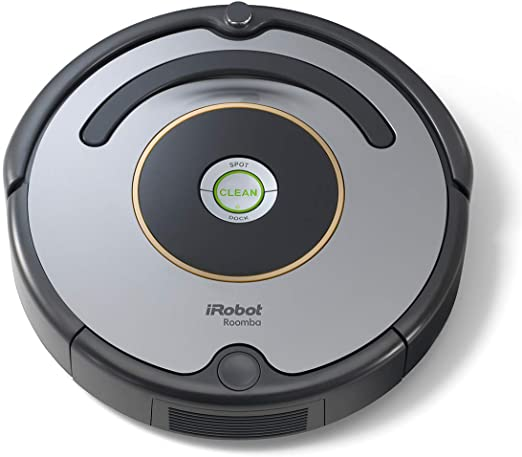
\includegraphics[width=\textwidth, height=\textwidth]{roomba.jpg}
    \caption{Roomba}
  \end{subfigure}
    \hfill
  \begin{subfigure}[b]{0.3\textwidth}
    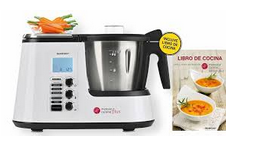
\includegraphics[width=\textwidth, height=\textwidth]{thermomix.png}
    \caption{Thermomix}
  \end{subfigure}
      \hfill
  \begin{subfigure}[b]{0.3\textwidth}
    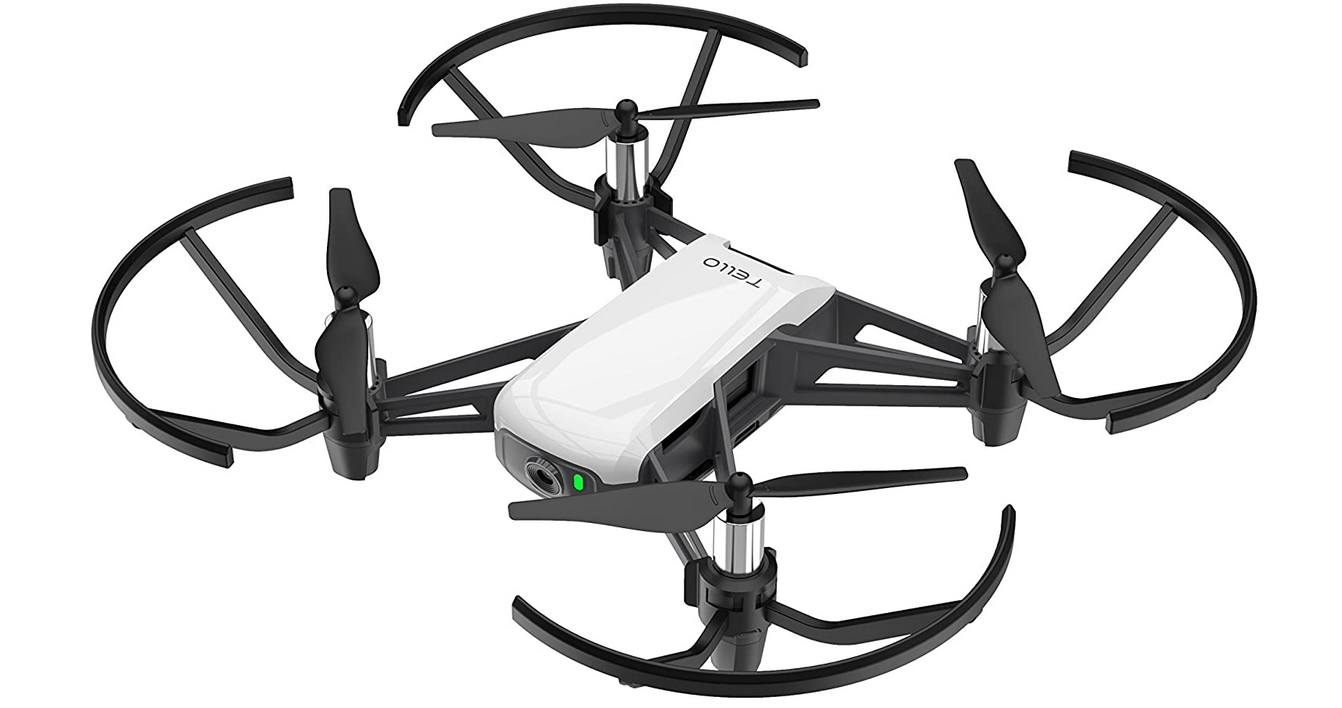
\includegraphics[width=\textwidth, height=\textwidth]{drone.png}
    \caption{Tello}
  \end{subfigure}
      \hfill
  \begin{subfigure}[b]{0.3\textwidth}
    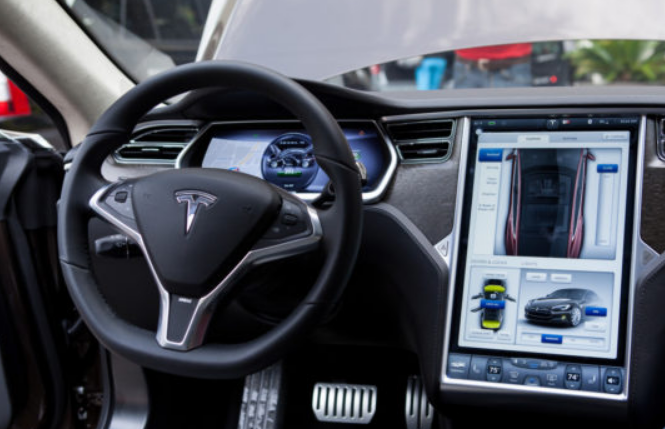
\includegraphics[width=\textwidth, height=\textwidth]{tesla.png}
    \caption{Tesla}
  \end{subfigure}
        \hfill
  \begin{subfigure}[b]{0.3\textwidth}
    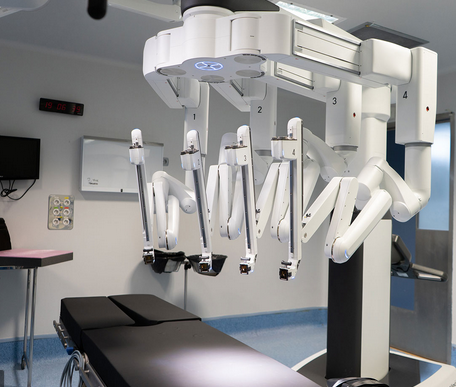
\includegraphics[width=\textwidth, height=\textwidth]{davinci.png}
    \caption{Robot DaVinci}
  \end{subfigure}
        \hfill
  \begin{subfigure}[b]{0.3\textwidth}
    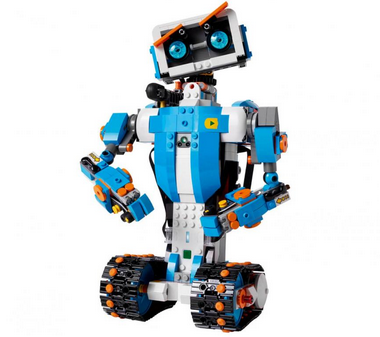
\includegraphics[width=\textwidth, height=\textwidth]{lego.png}
    \caption{Robots LEGO}
  \end{subfigure}
\caption{Ejemplos de robots en la actualidad}
\label{fig:EjemplosRobots}
\end{figure}


\section{Tecnologías web}
Las tecnologías web están en continuo desarrollo. Actualmente, existen tecnologías webtanto en el lado del cliente como en el lado del servidor. La idea de esta separación es marcar las diferentes partes de un sistema software para poder controlarlo de una forma más eficaz. Por este motivo, el \textit{frontend} recoge los datos o interactúa con el usuario final y el \textit{backend} procesa esos datos o sirve los contenidos. \newline

Hoy en día, son muy comunes las aplicaciones web que se basan en estas tecnologías. Las aplicaciones web basan su funcionamiento en un modelo cliente - servidor en el que el cliente se encarga de recoger los datos que introduce el usuario y el servidor los procesa. Gracias a ellas, se puede leer en el navegador web el correo electrónico, ver películas y series, leer el periódico, comprar productos, etc. Algunas de las aplicaciones web con más éxito en los últimos años son \textit{Gmail}, \textit{Spotify}, \textit{Netflix}, \textit{Amazon} o \textit{AliExpress}.

\begin{figure}[!h]
  \begin{subfigure}[b]{0.5\textwidth}
    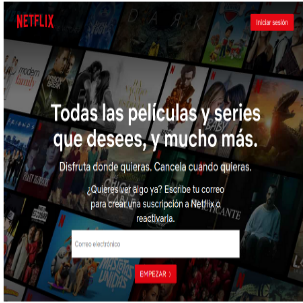
\includegraphics[width=\textwidth, height=\textwidth]{netflix.png}
    \caption{Dedicada a la distribución de contenidos}
  \end{subfigure}
        \hfill
  \begin{subfigure}[b]{0.5\textwidth}
    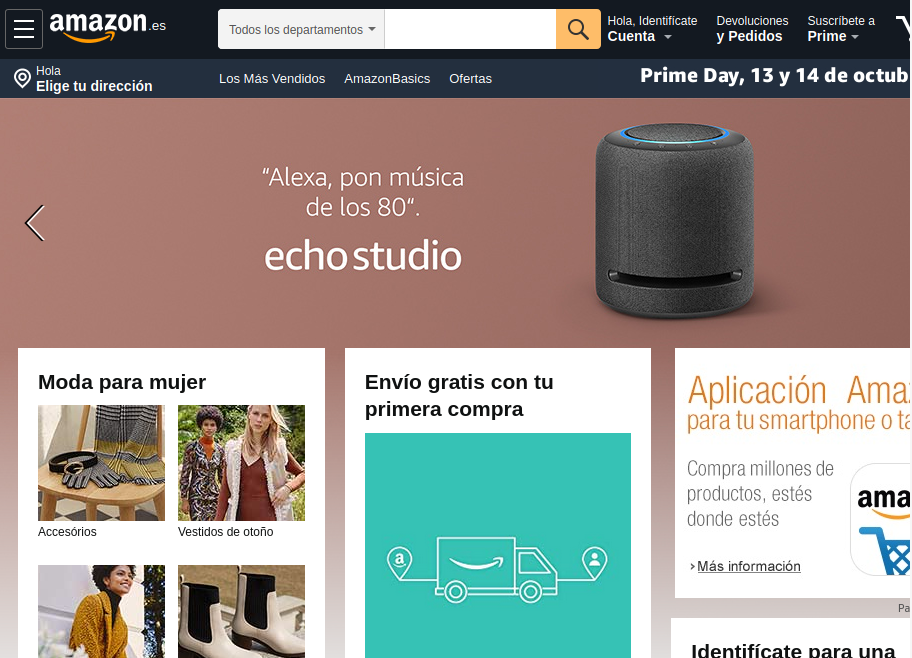
\includegraphics[width=\textwidth, height=\textwidth]{amazon.png}
    \caption{Dedicada a la venta online}
  \end{subfigure}
\caption{Ejemplos de aplicaciones web}
\label{fig:ejemplosaplicaciones}
\end{figure}

Por un lado, el \textit{frontend} engloba todas aquellas tecnologías web del lado del cliente que se encargan de recopilar los datos y mostrárselos al usuario. Principalmente, existen tres tecnologías de \textit{frontend}: \textit{HTML, CSS} y \textit{JavaScript}. Estas tres tecnologías permiten al usuario interactuar con el sevidor web, utilizando un navegador como intérprete. \newline 

Por otro lado, el \textit{backend} se encarga del almacenamiento de información en bases de datos, gestión de servidores y servir las vistas de las páginas web seleccionadas por el desarrollador en el lado del cliente o servir los contenidos multimedia. En el backend, el número de tecnologías es más extenso. La programación \textit{backend} incluye lenguajes como \textit{PHP, Python, Ruby, .NET o Java }y las bases de datos sobre las que se trabaja habitualmente pueden ser \textit{SQL, MongoDB o MySQL}. \newline 

La comunicación entre cliente y servidor se realiza utilizando el protocolo \textit{HTTP} (protocolo de transferencia de hipertexto). Este protocolo funciona mediante la emisión de una serie de peticiones y respuestas entre el cliente y el servidor usando diferentes métodos. Existen varios métodos \textit{HTTP}, los más comunes son los siguientes\footnote{https://developer.mozilla.org/es/docs/Web/HTTP/Methods}:

\begin{itemize}
    \item \textbf{GET}: solicitud de datos de un recurso concreto.
    \item \textbf{PUT}: reemplazo de las representaciones actuales del recurso de la petición.
    \item \textbf{POST}: envío de datos a un recurso concreto, normalmente provocando el cambio de estado del servidor.
    \item \textbf{DELETE}: eliminación de un recurso.
     \item \textbf{HEAD}: solicitud de datos de un recurso concreto tal y como ocurre con el método \textit{GET}, pero la respuesta no incluye cuerpo.
\end{itemize}

\begin{figure}[h!]
    \centering
    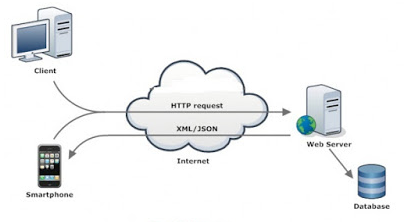
\includegraphics[scale=1]{http.png}
    \caption[Ejemplo de una interacción \textit{HTTP}]{Ejemplo de una interacción \textit{HTTP}\footnotemark} 
    \label{fig:http}
\end{figure}
\footnotetext{http://dsanchezzz.blogspot.com/2015/10/rest.html}

\clearpage
\subsection{Tecnologías web en el lado del cliente}
Las tres tecnologías web del \textit{frontend} que permiten la interacción entre usuario y servidor web son las siguientes:
\begin{itemize}
    \item \textit{HTML:} es un lenguaje de marcado que permite diferenciar los contenidos y definir la estructura de un sitio web. Permite dividir una página web en diferentes secciones: títulos, texto, imágenes, pie de página, etc. Es la base de toda página web. Sigue el modelo de objetos \textit{Document Object Model (DOM)}, que permite que el contenido de una página esté disponible para los programas en \textit{JavaScript}. Hoy en día, los navegadores emplean la versión \textit{HTML5}, que introduce como mejora las etiquetas de vídeo, de audio, de diálogos entre personas, de secciones y de bloques de contenidos.
    \item \textit{CSS}: es un lenguaje de hojas de estilo que permite modificar la apariencia de una página web. Gracias a este lenguaje, se puede organizar mejor el código al poder separar los datos (lenguaje \textit{HTML}) del diseño (lenguaje \textit{CSS}). Hoy en día, la versión disponible en los navegadores en \textit{CSS3}.
    \item \textit{JavaScript:} es un lenguaje de programación interpretado que permite definir el comportamiento de una página web (por ejemplo, al hacer click en un enlace). Por ello, gracias a este lenguaje el usuario puede interaccionar con la página web.
\end{itemize}

\subsection{Tecnologías web en el lado del servidor}
En el lado del servidor, algunas de las tecnologías que permiten acceder a bases de datos, escalabilidad, gestionar los servidores y servir las páginas web mediante la utilización de plantillas son:

\begin{itemize}
    \item \textit{Node.js}: uno de los lenguajes frecuentemente utilizado en la programación del \textit{backend} es el lenguaje \textit{JavaScript}. \textit{JavaScript} se creó para su uso en el \textit{frontend} en un principio; sin embargo, gracias al motor \textit{node.js}, este lenguaje puede ser interpretado en el lado del servidor sin necesidad de un navegador.
    \item \textit{Django}: es un entorno web de alto nivel programado en \textit{Python}. Es muy rápido y fácil de utilizar. Además, dispone de una interfaz para el manejo de las bases de datos \textit{SQL} y se puede acceder a ellas en el código mediante instrucciones \textit{Python}.
    \item \textit{Spring}: entorno basado en \textit{Java} que simplifica el desarrollo de aplicaciones. Facilita las tareas de configuración y el despliegue en el servidor.
\end{itemize}


\section{Docencia robótica}
Las tecnologías web ofrecen nuevas posibilidades para la robótica. Una de estas posibilidades es la docencia robótica. La docencia robótica ha estado creciendo en los últimos años gracias a que se trata de un campo de gran utilidad y que es una manera atractiva y divertida de introducir a los niños en la tecnología. Hoy en día existen muchas iniciativas para promover la docencia robótica. De hecho, ya se ha introducido en el currículum oficial de secundaria en muchas comunicades autónomas de España y en otros países del mundo.  \newline

En consecuencia, especialmente en los últimos años, han surgido algunas plataformas dedicadas a la docencia robótica que se encargan de impartir cursos de iniciación a la robótica desde edades muy tempranas para conseguir que los niños se sientan atraídos por esta rama desde el principio y aprendan a pensar como verdaderos programadores desde muy pequeños. \newline

La docencia robótica comparte los fundamentos de la educación \textit{STEM (Science, Technology, Engineering and Mathematics)}. Esta educación promueve el aprendizaje de la ciencia, tecnología, ingeniería y matemáticas y fomenta el desarrollo de un pensamiento crítico y la creatividad. \newline

Un ejemplo de estas plataformas que se comentan es el de \textit{Lenobotics}\footnote{https://lenobotics.com/}.  \textit{Lenobotics} es un programa que se encarga de impartir cursos de robótica en centros educativos para desarrollar las habilidades cognitivas de los niños que resultan necesarias para la programación. \newline

\clearpage
\begin{figure}[h!]
    \centering
    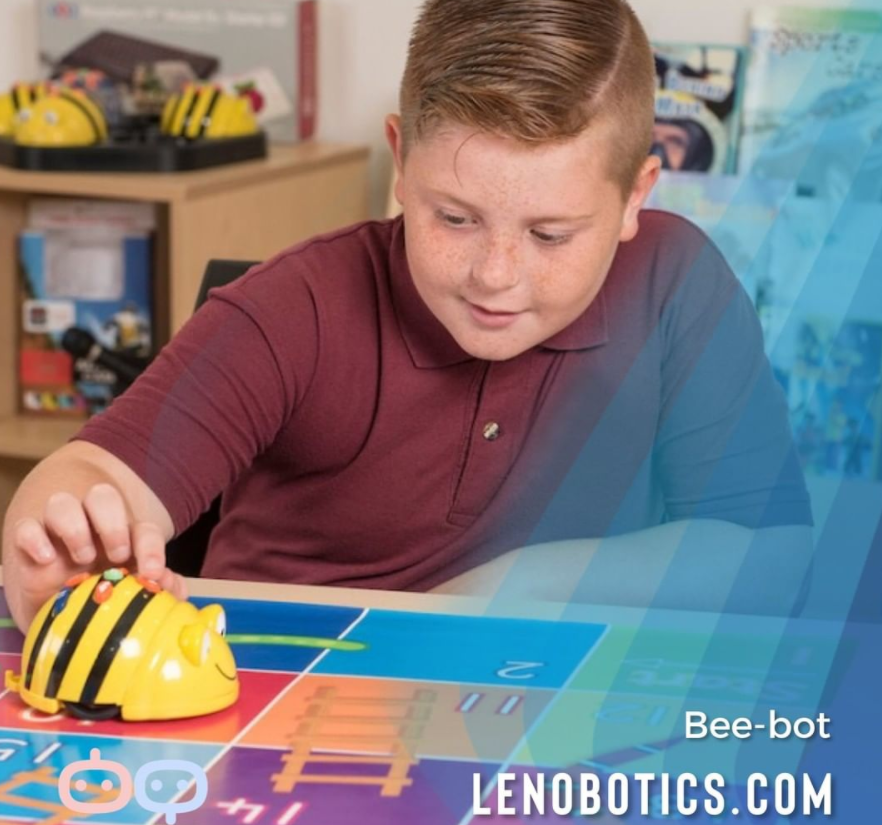
\includegraphics[scale=0.55]{lenobotics.PNG}
    \caption{Aprendizaje de programación robótica con \textit{Lenobotics}}
    \label{fig:lenobotics}
\end{figure}


Por su parte, \textit{LEGO education}\footnote{https://education.lego.com/es-es} también ofrece a los más pequeños la posibilidad de iniciarse en la robótica a través de sus kits. Estos kits permiten aprender unas primeras nociones de electrónica, robótica y programación. \newline

\begin{figure}[h!]
    \centering
    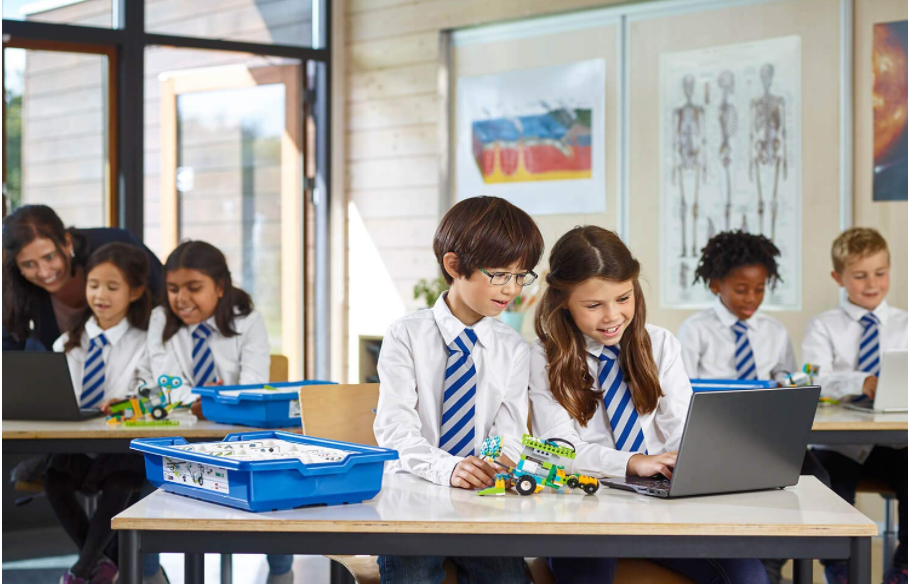
\includegraphics[scale=0.7]{lego.PNG}
    \caption{Aprendizaje de programación robótica con \textit{LEGO education}}
    \label{fig:lego}
\end{figure}

\clearpage
Otro ejemplo es el de \textit{OpenRoberta}\footnote{https://lab.open-roberta.org/}, que ofrece una interfaz de programación por medio de bloques de texto para diferentes modelos de robot. También dispone de una sección con ejercicios resueltos de muestra, para que los más inexpertos puedan empezar a familiarizarse con ellos.

\begin{figure}[h!]
    \centering
    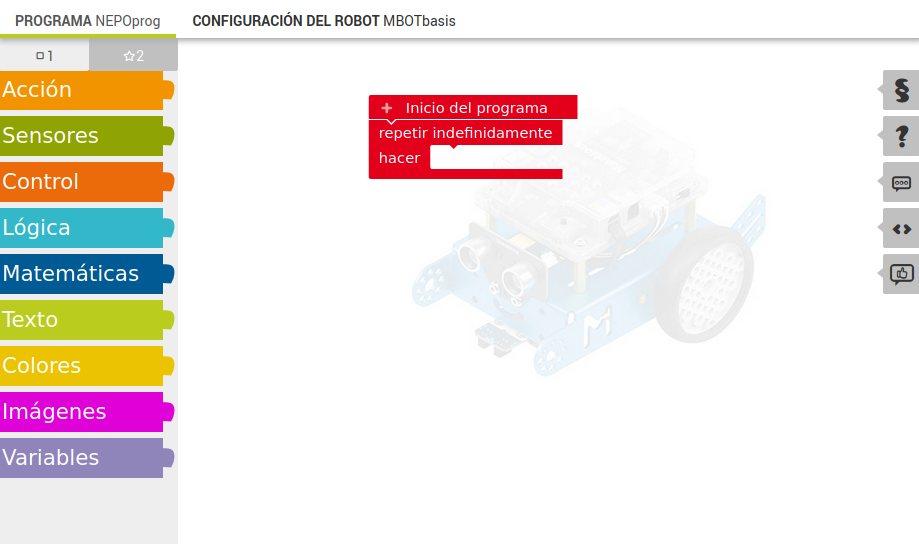
\includegraphics[scale=0.35]{openroberta.PNG}
    \caption{Aprendizaje de programación robótica con \textit{OpenRoberta}}
    \label{fig:lego}
\end{figure}

\textit{iRobot}\footnote{https://edu.irobot.com/} ofrece la posibilidad tanto de crear modelos de robot como de programar el cerebro de esos robots. Este entorno hace especial hincapié en la enseñanza \textit{STEM} como mejor método de aprendizaje de robótica.

\begin{figure}[h!]
    \centering
    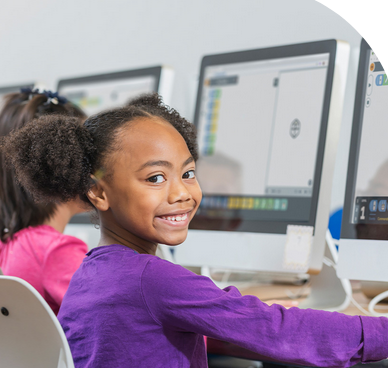
\includegraphics[scale=0.5]{irobot.PNG}
    \caption{Aprendizaje de programación robótica con \textit{iRobot}}
    \label{fig:lego}
\end{figure}

\textit{Scratch}\footnote{https://scratch.mit.edu/} es un lenguaje de programacion visual que fue desarrollado por el Grupo \textit{Lifelong Kindergarten del MIT Media Lab}. Hoy en día, se utiliza frecuentemente en la educación de ninos y adolescentes, ya que permite el aprendizaje de la programación sin tener un amplio conocimiento del código. Ofrece al usuario la posibilidad de programar construyendo una secuencia de código a partir de diversos bloques de acciones. El programador es capaz de construir la secuencia de
codigo con rapidez y facilidad, ya que cada bloque incluye una secuencia de texto que explica la función que desempeña. Por ello, la secuencia de código finalmente podrá ser leída e interpretada como si de un texto se tratase.

\begin{figure}[h!]
    \centering
    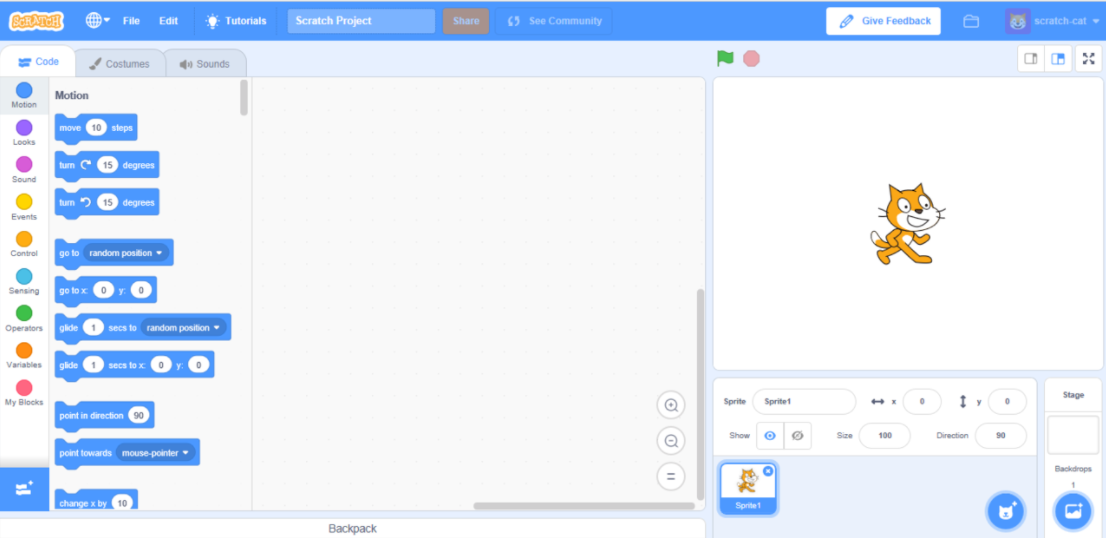
\includegraphics[scale=0.5]{scratch.PNG}
    \caption{Aprendizaje de programación robótica con \textit{Scratch}}
    \label{fig:scracth}
\end{figure}

El presente trabajo se va a centrar en la plataforma \textit{Kibotics}\footnote{https://kibotics.org/}, la cual es un entorno web para docencia en robótica y programación que permite a niños y adolescentes aprender programando. \textit{Kibotics}  apuesta por una enseñanza principalmente práctica, ya que resulta mucho más atractiva tanto la enseñanza como el aprendizaje de este modo que únicamente con clases teóricas. \newline

\textit{Kibotics}  se basa en la utilización del simulador \textit{WebSim}  que, a su vez, está basado en la tecnología \textit{A-Frame}  para representar los mundos. Este simulador permite la creación de romdiferentes ejercicios para los robots que tienen soporte en la plataforma: piBot, mBot, fórmula 1 y drone Tello. Estos ejercicios podrán solucionarse tanto en lenguaje \textit{Scratch} (especialmente indicado para aquellos alumnos que no hayan programado anteriormente) como en lenguaje \textit{Python}\footnote{https://es.python.org/} (para aquellos niños que cuenten con nociones previas). \newline

\begin{figure}[h!]
    \centering
    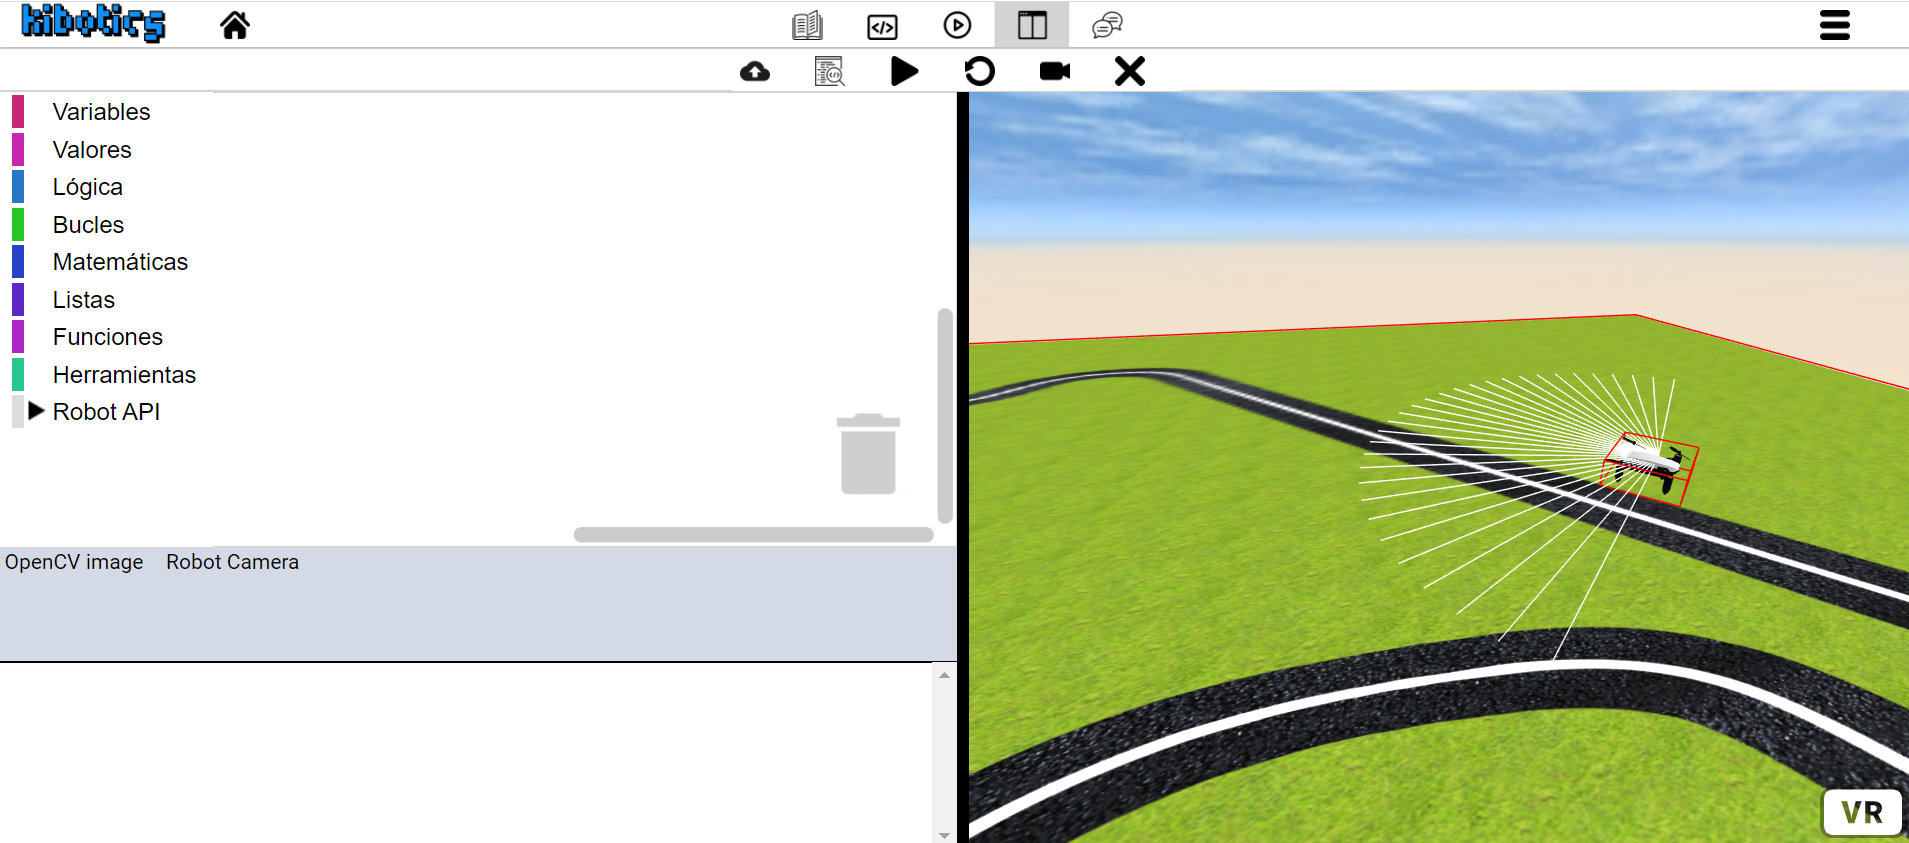
\includegraphics[scale=0.5]{kibotics.PNG}
    \caption{Interfaz de programación en \textit{Kibotics} de un ejercicio en \textit{Scratch}}
    \label{fig:kibotics}
\end{figure}

Muchos robots cuentan con cámaras incorporadas en el hardware, lo que permite la creación de ejercicios que se deben solucionar mediante la utilización de la visión artificial además de los ejercicios que se puedan solucionar mediante el uso de los sensores de los robots (sensores infrarrojos, por ejemplo). La Figura \ref{fig:RobotsKibotics} muestra los robots que soporta actualmente la plataforma.\newline


\begin{figure}[h!]
  \begin{subfigure}[b]{0.2\textwidth}
    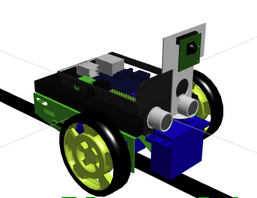
\includegraphics[width=\textwidth, height=\textwidth]{pibot.png}
    \caption{piBot}
  \end{subfigure}
  \hfill
  \begin{subfigure}[b]{0.2\textwidth}
    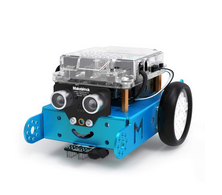
\includegraphics[width=\textwidth, height=\textwidth]{mbot.png}
    \caption{mBot}
  \end{subfigure}
    \hfill
  \begin{subfigure}[b]{0.2\textwidth}
    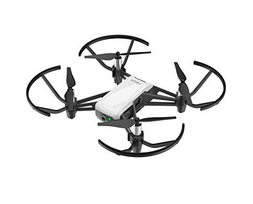
\includegraphics[width=\textwidth, height=\textwidth]{tello_2.png}
    \caption{Drone Tello}
  \end{subfigure}
    \hfill
  \begin{subfigure}[b]{0.2\textwidth}
    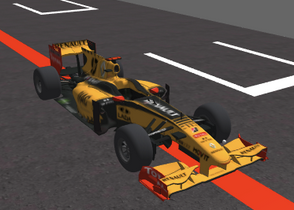
\includegraphics[width=\textwidth, height=\textwidth]{f1.png}
    \caption{Fórmula 1}
  \end{subfigure}
\caption{Robots soportados en la plataforma \textit{Kibotics}}
\label{fig:RobotsKibotics}
\end{figure}


Por último, cabe destacar la importancia de los motores de físicas que incorporan los simuladores robóticos usados tanto en docencia como en investigación robótica. Un motor de físicas es un software capaz de realizar simulaciones de ciertos sistemas físicos como la dinámica del cuerpo en movimiento, la fricción y la elasticidad de una colisión. Se emplean con mucha frecuencia en los videojuegos, para recrear con un mayor realismo el movimiento de los personajes. \newline

Existen numerosos motores de físicas como \textit{Box2D}\footnote{https://box2d.org/} (simulaciones 2D), \textit{Cocos2D,}\footnote{https://www.cocos.com/} (simulaciones 2D) \textit{Ammo.js}\footnote{https://github.com/kripken/ammo.js/} (simulaciones 3D) o \tetxit{CANNON}\footnote{http://schteppe.github.io/cannon.js/} (simulaciones 3D). El presente trabajo se va a centrar en este último, ya que es el que emplea \textit{A-Frame} en la actualidad. \\ En el capítulo 3, se explicará con mayor detalle las peculiaridades de este motor de físicas en cuestión. 



% OBJETIVOS %
%%%%%%%%%%%%%%%%%%%%%%%%%%%%%%%%%%%%%%%%%%%%%%%%%%%%%%%%%%%%%%%%%%%%%%%%%%%%%%%%
\chapter{Objetivos}
\label{chap:objetivos} 
En este capítulo se explican los objetivos del presente trabajo, la metodología que se ha seguido para alcanzarlos y la planificación que se ha llevado durante el proceso de desarrollo.
   
\section{Objetivos}
En los mundos de los simuladores que se emplean en docencia robótica hay objetos estáticos, móviles y los propios robots programados por los niños. Los objetivos que persiguen este trabajo son los siguientes:

\begin{itemize}
    \item Desarrollar un motor de físicas basado en \textit{A-Frame} que permita replicar de modo realista el movimiento autónomo de los robots programados por los estudiantes de la plataforma \textit{Kibotics} y que se complemente con \textit{CANNON}, el motor por defecto que materializa la gravedad, rozamiento y los choques.
    \item Crear varios ejercicios en la plataforma educativa \textit{Kibotics} que saquen partido del nuevo motor de físicas y sean vistosos, incluyendo sus escenarios y que sirvan de validación experimental.
\end{itemize}

Además, estos objetivos deben satisfacerse cumpliendo los siguientes requisitos:

\begin{itemize}
    \item Materialización de robots con distinta masa y un movimiento autónomo realista, con una aceleración máxima limitada y capacidad de control acotada.
    \item Coexistencia con el motor por defecto \textit{CANNON} que no requiera la modificación de su código fuente.
\end{itemize}

\section{Metodología}
Con el fin de asegurar el correcto desarrollo del Trabajo de Fin de Grado se estableció una reunión semanal con el tutor para compartir los progresos realizados durante la semana y en la que el tutor me pudo orientar sobre dónde dirigir los esfuerzos. Paralelamente a las reuniones semanales, también se ha contado con un canal de slack en el que se encuentran todos los contribuyentes de la plataforma \textit{Kibotics} donde se han podido plantear todo tipo de dudas durante el proceso de aprendizaje. \newline


También se ha elaborado un blog en el que se han ido compartiendo los resultados y el trabajo que se ha realizado cada semana. El blog se ha implementado gracias al dominio gratuito que ofrece GitHub para crear un blog\footnote{https://roboticslaburjc.github.io/2019-tfg-natalia-monforte/} basado en GitHub Pages. En el README de mi Github se ha incluido un enlace pinchable para acceder a dicho blog\footnote{https://github.com/RoboticsLabURJC/2019-tfg-natalia-monforte}. \newline

El modelo de desarrollo software seleccionado ha sido el método en cascada. En primer lugar, se han ido marcando subobjetivos de implementación. Después de finalizar un subobjetivo, se pasaba a una fase de verificación de las funcionalidades y corrección de errores tras la cual se reanudaba el proceso de desarrollo. Las fases en las que se ha dividido la implementación realizada han sido: 

\begin{itemize}
    \item Implementación del movimiento lineal del drone (eje vertical).
    \item Implementación del movimiento lineal para robots terrestres en el plano horizontal.
    \item Implementación de la estabilización del drone cuando se encuentra inmóvil durante el vuelo.
    \item Implementación del movimiento angular para robots terrestres y drones.
\end{itemize}

Para integrar el código de las mejoras o aportaciones realizadas al código fuente de la plataforma \textit{Kibotics}, cabe destacar que se ha utilizado el sistema que ofrece GitHub para integrar código mediante la creación de incidencias, de nuevas ramas y de parches. Para que los desarrolladores pudiesen añadir las nuevas funcionalidades al código fuente oficial de \textit{Kibotics}, se creaba una nueva rama actualizada con los últimos cambios de la rama
principal. Sobre esta rama se desarrollaba la solución a cada incidencia. Una vez incluidos los cambios se explicaban en un comentario o parche y se subían a la nueva rama creada del repositorio de \textit{Kibotics}. El siguiente paso consistía en solicitar la fusión de los cambios de esta rama con
la rama principal, abriendo peticiones \textit{pull request}. Tras la solicitud de la fusión del parche los desarrolladores que cuentan con más experiencia verifican que los cambios son correctos y, si es así, integran los cambios a la rama maestra oficial, dando por resuelta la incidencia. Los comandos necesarios para realizar la integración del código a la rama creada son los siguientes: 

\begin{verbatim}
                git checkout -b issue-XXX
                git add -ruta-del-fichero-a-añadir
                git commit -m "Comentario para el commit"
                git push -u origin issue-XXX
\end{verbatim}

\section{Plan de trabajo}
El proceso de elaboración del Trabajo de Fin de Grado se ha divido en cinco fases distintas:
\begin{itemize}
    \item \textbf{FASE 1:} aprendizaje y primera toma de contacto con las tecnologías web necesarias para la elaboración del trabajo. Especialmente \textit{A-Frame y JavaScript}.
    \item \textbf{FASE 2:} estudio del código de \textit{Kibotics-WebSim} y de las físicas de \textit{A-Frame} (motor de \textit{CANNON}).
    \item \textbf{FASE 3:} Elaboración de un motor de físicas complementario para el simulador \textit{WebSim}.
    \item \textbf{FASE 4:} creación de los primeros mundos utilizando las funcionalidades proporcionadas por \textit{Blender y A-Frame} y creación de nuevos ejercicios para incluir en la plataforma.
\end{itemize}

% HERRAMIENTAS %
%%%%%%%%%%%%%%%%%%%%%%%%%%%%%%%%%%%%%%%%%%%%%%%%%%%%%%%%%%%%%%%%%%%%%%%%%%%%%%%%
\chapter{Herramientas}
\label{chap:herramientas} 
En este capítulo se explica con un mayor grado de detalle qué herramientas han sido necesarias para el desarrollo del trabajo. Principalmente, se han utilizado los lenguajes de programación \textit{JavaScript, HTML, JSON, Python y Scratch}. Por otro lado, se han utilizado aplicaciones como \textit{Blender} para el modelado de objetos 3D y el simulador \textit{WebSim} para la recreación de los mundos tridimensionales.
   
\section{Lenguaje \textit{JavaScript}}
\textit{JavaScript} es un lenguaje de programación interpretado de alto nivel que se encuentra bajo el estándar \textit{ECMAScript}\footnote{Especificación de lenguaje de programación en el que se definen tipos dinámicos y soporte de programación oreintada a objetos}. Este lenguaje es comúnmente conocido por su uso en los scripts de las páginas web. No obstante, dada su orientación a objetos y a ser un lenguaje de programación basada en prototipos y de un solo hilo, es usado en otros muchos entornos externos de la página web: \textit{Node.js, Apache CouchDB o Adobe Acrobat}\footnote{https://developer.mozilla.org/es/docs/Web/JavaScript}. \newline

La sintaxis es similar a la utilizada en \textit{Java} y \textit{C++}. De esta manera, se facilita el aprendizaje del lenguaje ya que está basado en conceptos ya conocidos por el programador. Las estructuras del lenguaje, tales como sentencias condicionales (if y switch) y bucles (while y for), funcionan de una manera similar a como lo hacen en otros lenguajes de programación\footnote{\textit{https://developer.mozilla.org/es/docs/Web/JavaScript}}. \newline

Las siguientes características son las principales:
\begin{itemize}
    \item Lenguaje escructurado similar a la estructura utilizada en \textit{Java} y \textit{C++}.
    \item \textit{ECMAScript 2015} añadió la palabra clave \textit{let}, que permite que el alcance de la variable se corresponda con el bloque en el que esta se haya definido (\textit{block scoping}).
    \item Tipado débil, es decir, el tipo de datos se asocia al valor de la variable en un preciso momento.
    \item El lenguaje está formado por objetos.
    \item Lenguaje interpretado, es decir, se compila justo-a-tiempo. No es necesario disponer de un compilador adicional, cada navegador incluye un intérprete que se encarga de ejecutar el código.
\end{itemize}

Este TFG está enteramente programado en \textit{JavaScript}, ya que se trata de una aplicación web que corre en el lado del cliente. 

\section{Lenguaje \textit{HTML}}
\textit{HTML} es un lenguaje de marcado que define la estructura de una página web. \textit{HTML} ofrece una serie de elementos que permiten etiquetar diferentes partes de una misma página web en una misma clase para otorgarles una misma apariencia. Además, \textit{HTML} permite cambiar el estilo de las palabras (por ejemplo, a cursiva, a negrita, agrandar o reducir el tamaño de letra, etc)\footnote{https://developer.mozilla.org/es/docs/Learn/Getting$_$started$_$with$_$the$_$web/HTML$_$basics}. \newline

Las partes principales del elemento \textit{HTML} son las siguientes:
\begin{itemize}
    \item \textbf{Etiqueta de apertura:} se trata del nombre del elemento y se incluye entre paréntesis angulares $(< >)$. Indica el inicio del elemento.
    \item \textbf{Etiqueta de cierre:} similiar a la etiqueta de apertura salvo que incluye, además, una barra de cierre (/) precediendo al nombre de la etiqueta. Indica el fin del elemento.
    \item \textbf{Contenido: }todo aquello que se incluye entre la etiqueta de apertura y la de cierre.
    \item \textbf{Elemento: }es el conjunto formado por las etiquetas de apertura y cierre y el contenido del elemento.
\end{itemize}

Las etiquetas básicas de \textit{HTML} son la siguientes:
\begin{itemize}
    \item $<html>.$: comienzo del documento HTML.
    \item $<head>.$: cabecera de la página.
    \item $<body>.$:  cuerpo de la página.
    \item $<h1>, <h2>, etc.$: son los títulos o encabezados.
    \item $<a>.$: define los enlaces.
    \item $<table>.$: es una tabla.
    \item $<p>.$: define un párrafo.
    \item $<img>.$: imágenes.
    \item $<ul>.$: define una lista.
\end{itemize}

   


Además, cada elemento puede incluir uno o más atributos que permiten añadir mas información acerca de ese elemento. Por ejemplo, añadir información sobre el estilo del elemento. A continuación, se incluye un fragmento de código \textit{HTML} a modo de ejemplo. 
\begin{verbatim}







<!DOCTYPE html>
<html>
  <head>
    <meta charset="utf-8">
    <title>Mi código de prueba</title>
  </head>
  <body>
    <p class="editor-note">Esto es<strong>una prueba</strong></p>
  </body>
</html>
\end{verbatim}

\textit{Kibotics} emplea \textit{HTML} para crear las plantillas de las diferentes páginas que sirve la aplicación web.

\section{Lenguaje \textit{JSON}}
El acrónimo \textit{JSON} significa JavaScript Object Notation (Notación de Objetos de JavaScript). Se trata de un formato para el intercambio de datos. Es un lenguaje sencillo para la escritura y lectura humana y, al mismo tiempo, resulta fácil para las máquinas interpretarlo y procesarlo. \textit{JSON} está constituído por dos estructuras: una colección de pares nombre - valor y una lista ordenada de valores. Dado que estas convenciones son conocidas por otros lenguajes como  \textit{C, C++, C#, Java, JavaScript, Perl, Python}, se trata de un lenguaje ideal para el intercambio de datos\footnote{https://www.json.org/json-es.html}. \newline

\clearpage
En \textit{JSON}, estas estrucutras se presentan de la siguiente forma:
\begin{itemize}
    \item \textbf{Objeto: } conjunto desordenado de pares nombre - valor. Un objeto va encerrado entre llaves ({ }). La sintaxis es la siguiente: 
    \begin{verbatim}
        objeto {
            nombre1: valor1,
            nombre2: valor2,
            ...
        }
    \end{verbatim}
    \item \textbf{Array: } colección de valores. Van encerrados entre corchetes [ ]. Un valor puede ser una cadena de caracteres con comillas dobles, un número, true, false o null, un objeto o un array. Estas estructuras pueden anidarse.

\end{itemize}

La plataforma \textit{Kibotics} emplea \textit{JSON} para los ficheros de configuración de los diferentes escenarios utilizados en los ejercicios que ofrece la aplicación. Mediante un \textit{parser} se recopila la información necesaria del fichero de configuración \textit{JSON} para construir el mundo en \textit{A-Frame}.

\section{\textit{Blender}}
\textit{Blender}\footnote{https://www.blender.org/} es un programa informático multi plataforma, es decir, compatible para distintos sistemas operativos como Windows o Linux. Las funciones principales que se pueden realizar con \textit{Blender} son el modelado, iluminación, renderizado, animación y creación de gráficos tridimensionales. También se pueden realizar actividades relacionadas con la composición de vídeo. 

\begin{figure}[h!]
    \centering
    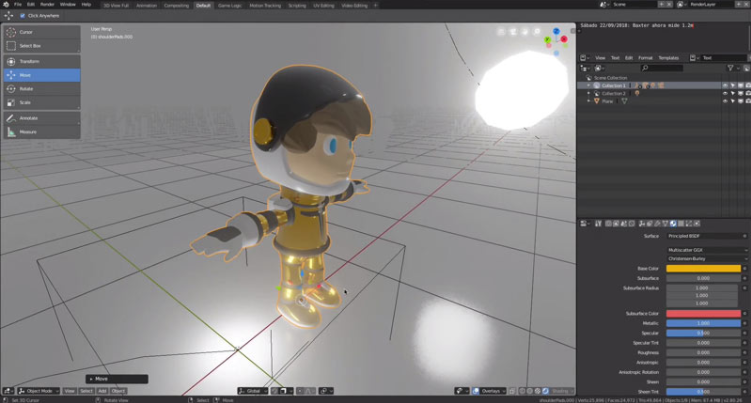
\includegraphics[scale=0.7]{blender.PNG} 
    \caption{Interfaz de trabajo con \textit{Blender}}
    \label{fig:blender}
\end{figure}

Durante el presente trabajo se ha utilizado esta herramienta para modificar la rotación y apariencia de los robots de los que dispone la plataforma \textit{Kibotics}. Además, \textit{Blender} permite exportar los modelos en formato glTF (GL Transmission Format). glTF es un formato de archivo basado en el estandar \textit{JSON}. Permite la compresión de escenas y modelos 3D para minimizar el tiempo de ejecución de los programas en los que posteriormente se utilicen.

\section{Entorno \textit{A-Frame}}
A-Frame es un marco web para crear escenas de realidad virtual en el navegador. Ha sido utilizado por empresas como \textit{Google, Disney, Samsung, Toyota} o \textit{CERN}, entre otras. Además, algunas de ellas, como \textit{Google, Microsoft, Oculus} y \textit{Samsung} han llegado a realizar contribuciones. Sus principales características son las siguientes\footnote{https://aframe.io/docs/1.0.0/introduction/#features}:

\begin{itemize}
    \item \textbf{Permite un uso sencillo de la realidad virtual:} para usar \textit{A-Frame} basta con colocar las etiquetas $<script>$ y $<a-scene>$. A-Frame se encarga del modelado 3D y la realidad virtual, no es necesaria la instalación de ningún paquete externo.
    \item \textbf{\textit{HTML} declarativo:} \textit{A-Frame} está basado en \textit{HTML}, por ello es fácil y accesible para cualquier programador, puesto que HTML es un lenguaje ampliamente conocido.
    \item \textbf{Arquitectura de componente de entidad:} \textit{A-Frame} sigue el patrón \textit{ECS} (entidad-componente-sistema). Se trata de un patrón de desarrollo de juegos basado en el principio de composición sobre herencia. De esta manera, se otorga una mayor flexibilidad en la definición de entidades ya que cada objeto de la escena se corresponde con una entidad y cada entidad, a su vez, está compuesta por uno o más componentes que contienen datos y estado de la entidad. Por tanto, una entidad puede verse modificada en tiempo de ejecución si alguno de los componentes que agrega modifica sus datos.
    \item \textbf{Multiplataforma: } \textit{A-Frame} es compatible con plataformas tan variadas como \textit{Vive, Rift, Windows Mixed Reality, Daydream, GearVR y Cardboard}.
    \item \textbf{Rendimiento:} las actualizaciones de \textit{A-Frame} se realizan en la memoria y con poco gasto energético. A-Frame se encuentra optimizado para \textit{WebVR}.
    \item  \textbf{Inspector visual:} \textit{A-Frame} cuenta con un inspector visual integrado. Este se despliega al presionar la combinación de teclas $<ctrl>$ + $<alt>$ + $i$. El inspector permite detectar el origen de problemas o desarrollar una mejor distribución de la escena con menos esfuerzo.
    \item \textbf{Componentes:} \textit{A-Frame} cuenta con una gran cantidad de componentes con los que trabajar. Esta amplia variedad va desde componentes geométricos básicos o materiales hasta componentes como la teletransportación, la realidad aumentada o componentes personalizados por el usuario.
\end{itemize}

\begin{figure}[h!]
    \centering
    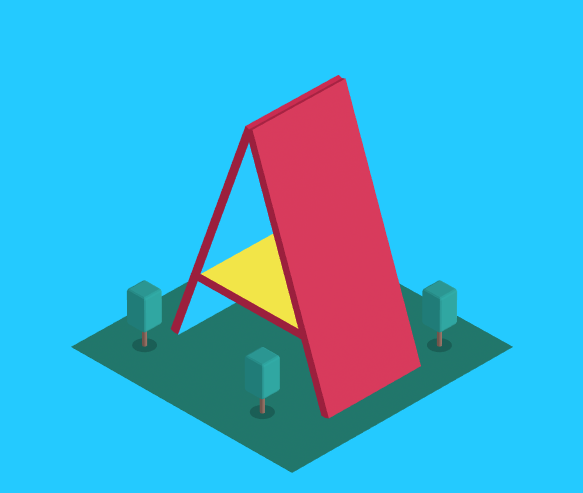
\includegraphics[scale=0.75]{a-frame.PNG} 
    \caption[Ejemplo de construción 3D con \textit{A-Frame}]{Ejemplo de construción 3D con \textit{A-Frame} \footnotemark}
    \label{fig:a-frame}
\end{figure}
\footnotetext{https://aframe.io/}

\subsection{Sistema de físicas de \textit{A-Frame}}
Las físicas de \textit{A-Frame} soportan dos motores de físicas: \textit{Ammo Driver y CANNON}. Actualmente, el motor que está en uso por defecto es el de \textit{CANNON}\footnote{https://github.com/donmccurdy/aframe-physics-system}. No obstante, ya ha sido añadido el soporte de \textit{Ammo.js} al sistema de físicas, y se preveé que \textit{CANNON} acabe quedando obsoleto con el paso del tiempo. \newline

Para la instalación del sistema de físicas de \textit{A-Frame} basta con incluir el siguiente script en el código \textit{HTML} de la aplicación: 

\begin{verbatim}
<script src="//cdn.rawgit.com/donmccurdy/aframe-physics-system/v4.0.1/  
dist/aframe-physics-system.min.js"></script>
\end{verbatim}

El sistema de físicas de \textit{A-Frame} cuenta con dos tipos de cuerpos: dinámicos y estáticos.

\begin{itemize}
    \item \textbf{Cuerpo dinámico:} aquellos objetos de la escena que presentan libertad de movimiento. Estos objetos se ven afectados por la gravedad, la fricción y las colisiones.
    \item \textbf{Cuerpo estático:} aquellos objetos de la escena que no necesitan modificar su posición en la misma. Son cuerpos fijos y sin animaciones. Otros cuerpos dinámicos podrán colisionar con un cuerpo estático, pero el cuerpo estático no verá modificada su posición tras la colisión.
\end{itemize}

El sistema de físicas ofrece la posibilidad de añadir una malla de colisión a un objeto de la escena. Existen mallas de colisión de diferentes formas, por lo que se debe seleccionar aquella que se ajuste mejor al objeto en cuestión. Se puede elegir entre el ajuste automático, una caja, un cilindro, una esfera, un cuerpo convexo o una primitiva ( plano, cilindro o esfera seleccionadas automáticamente en función de la primitiva \textit{A-Frame} correspondiente). \newline


Cada escena de  \textit{A-Frame}  admite una serie de parámetros a los que se les puede modificar el valor para ajustar el mundo a las características deseadas. Si no se especifica el valor que se desea de un parámetro, este tomará el valor por defecto. Algunos de los parámetros que admite una escena son \textit{debug}, que cuando está a \textit{true} muestra las mallas de colisión de los objetos de la escena o \textit{gravity, friction y restitution}, que se corresponden con la gravedad, fricción y coeficiente de restitución, respectivamente, del mundo simulado.
\begin{table}[h!]
\centering
\begin{tabular}{|c|c|}
\hline
\textbf{Atributo}    & \textbf{Valor por defecto} \\ \hline
debug       & true              \\ \hline
gravity     & -9.8              \\ \hline
friction    & 0.01              \\ \hline
restitution & 0.3               \\ \hline
\end{tabular}
\caption{Parámetros configurables del sistema de físicas de \textit{A-Frame}}
\label{fig:param-fisicas}
\end{table}

\section{Plataforma \textit{Kibotics}}
La batería de ejercicios que incluye el entorno \textit{Kibotics} se ejecuta usando el simulador robótico \textit{Websim}. Se trata de un simulador diseñado para el aprendizaje de conceptos básicos de programación de robots especialmente para niños. El simulador permite que los usuarios puedan programar fácilmente los movimientos de los robots, ya que simplemente tienen que acceder a la información que recogen sus sensores y enviar las órdenes precisas a los actuadores del robot. Estas órdenes se deberán programar, en\textit{ Python o Scratch}, dentro del editor que incorpora la interfaz de \textit{Websim}. \newline

El simulador está diseñado basándose en el uso del entorno \textit{A-Frame}. A su vez, \textit{A-Frame} se sirve del motor de físicas de \textit{CANNON} para materializar los movimientos de los cuerpos dinámicos en la escena.

\begin{figure}[h!]
    \centering
    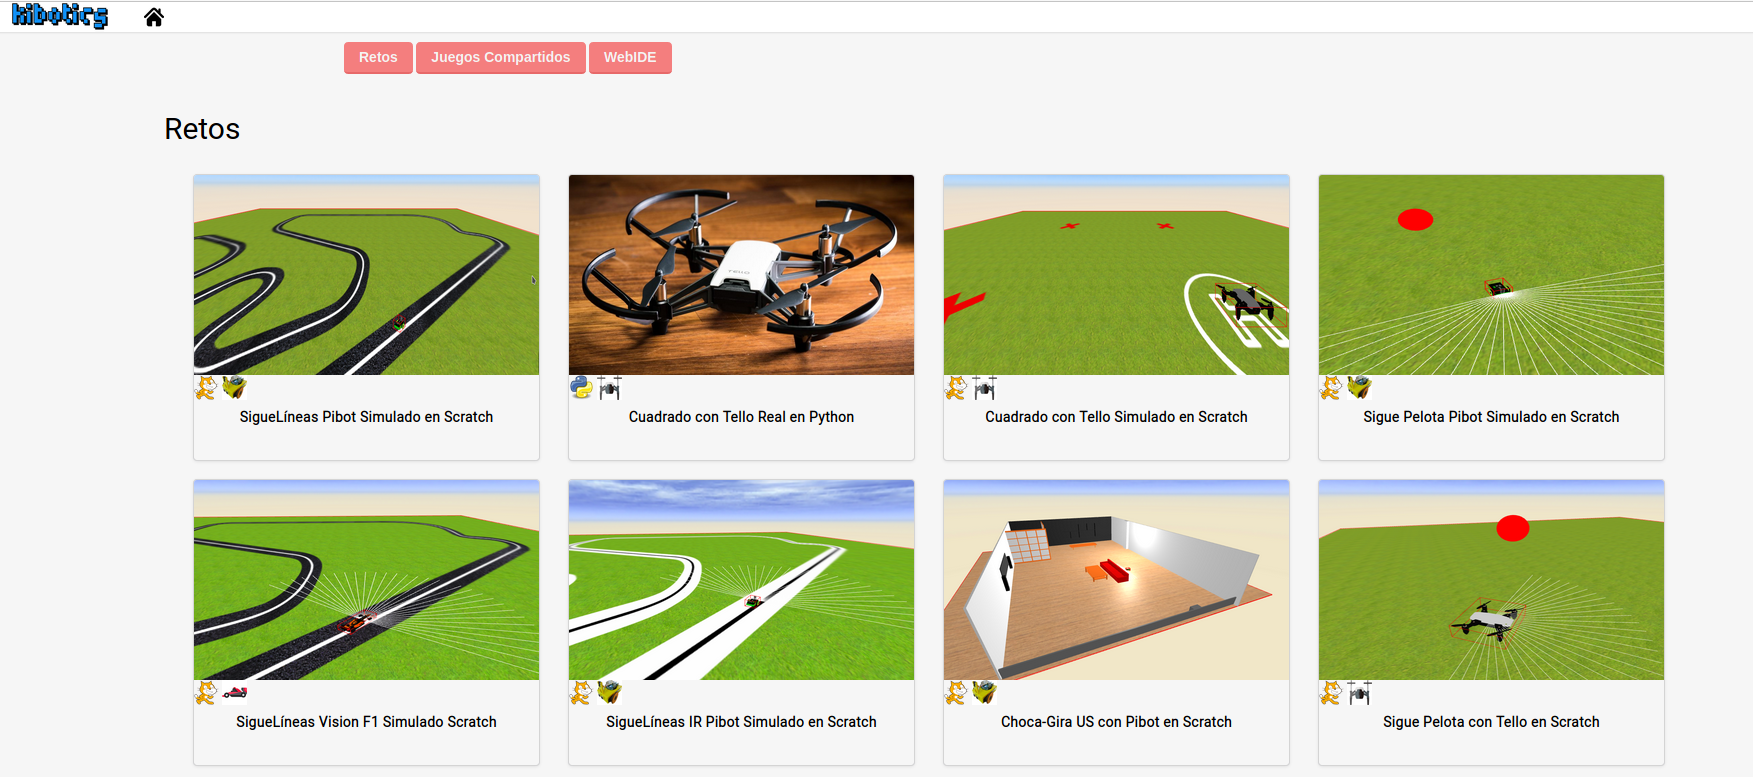
\includegraphics[scale=0.25]{kibotics.png} 
    \caption{Menú de ejercicios de \textit{Kibotics}}
    \label{fig:kibotics}
\end{figure}

\begin{figure}[h!]
    \centering
    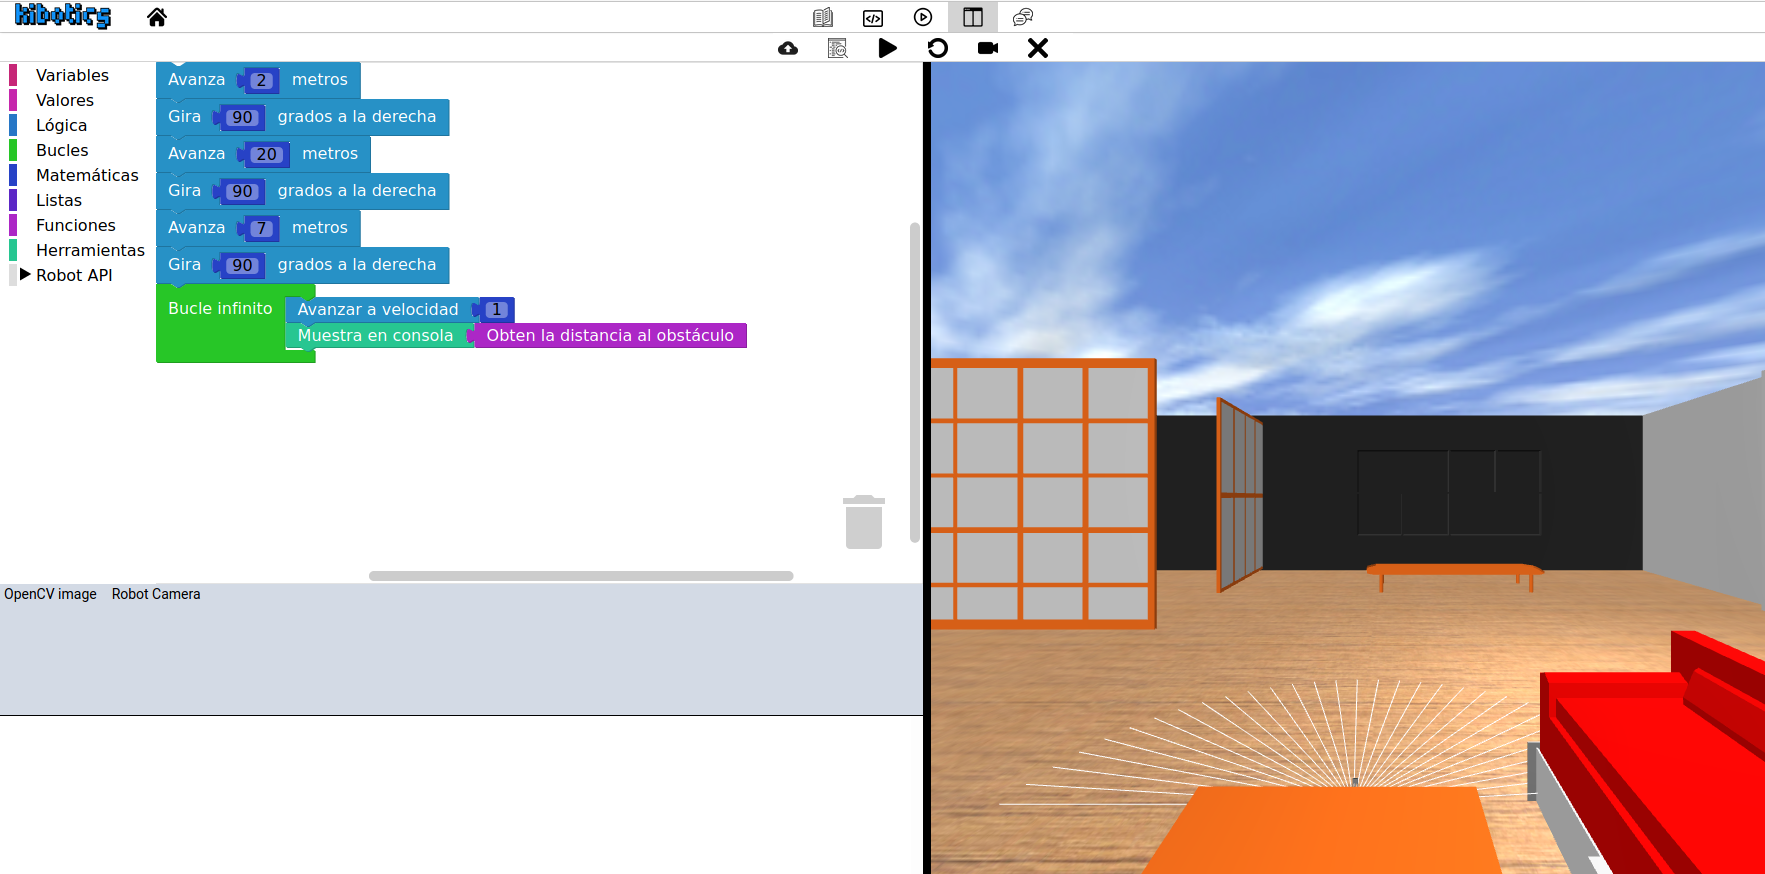
\includegraphics[scale=0.25]{scratch.png} 
    \caption{Editor \textit{Scratch} en \textit{WebSim}}
    \label{fig:scratch}
\end{figure}

\begin{figure}[h!]
    \centering
    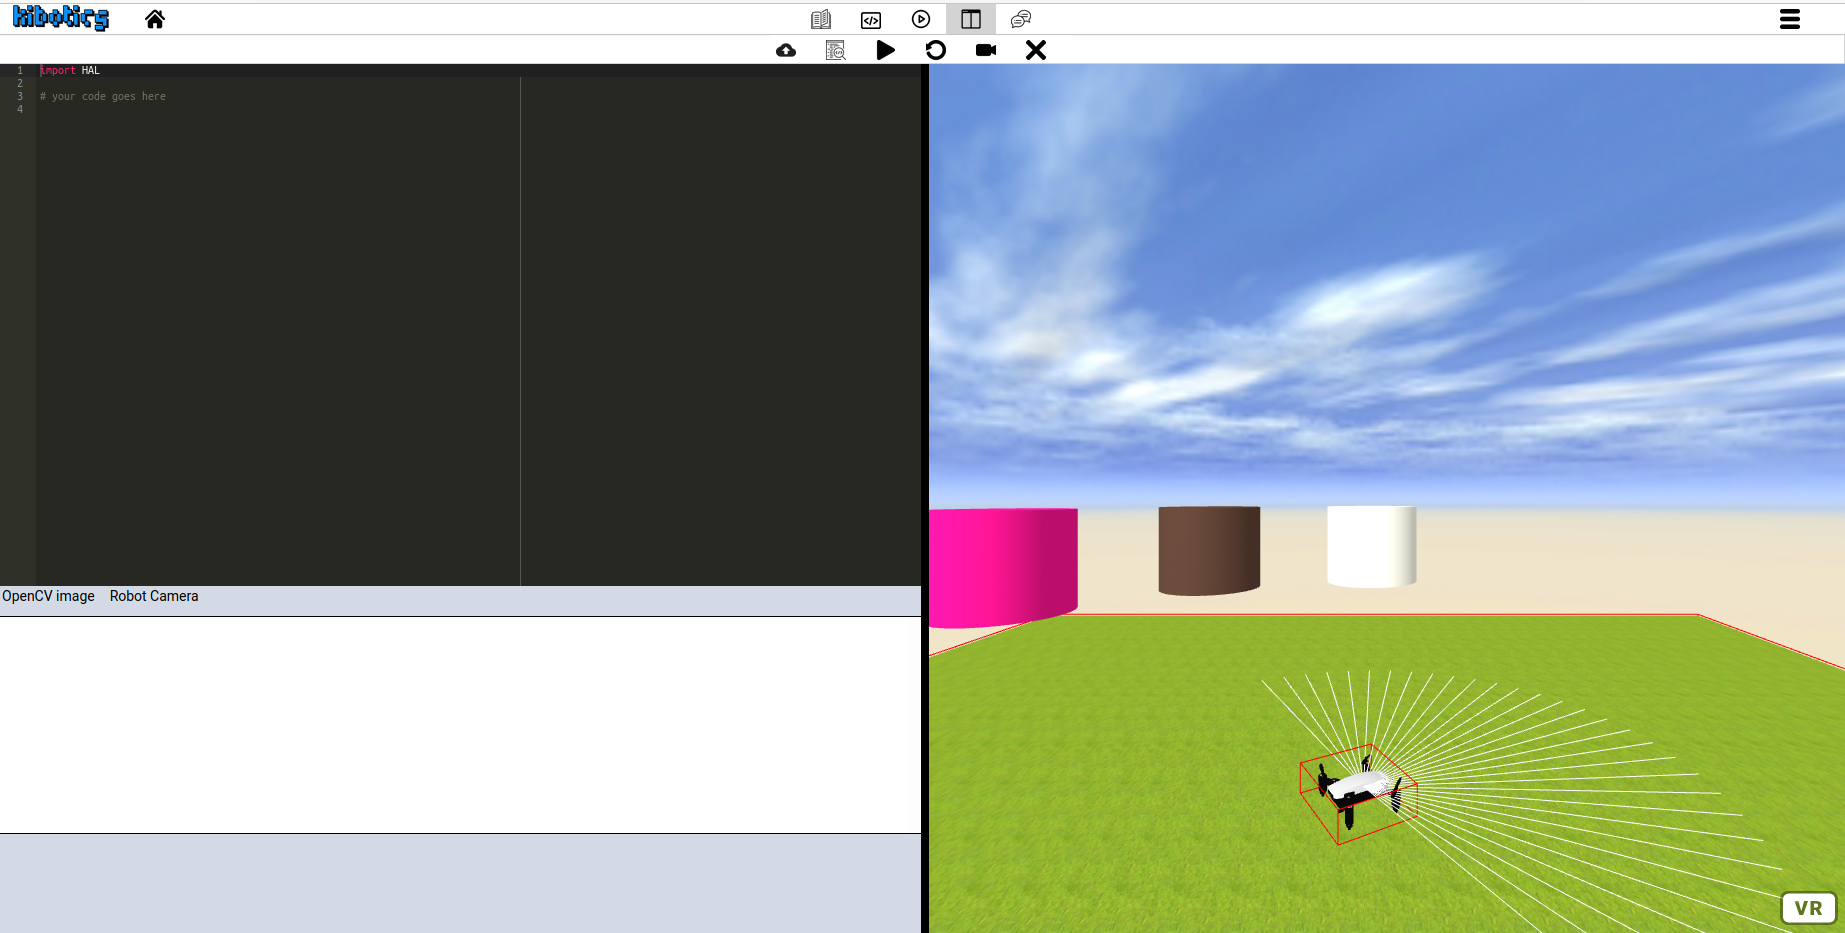
\includegraphics[scale=0.25]{python.png} 
    \caption{Editor \textit{Python} en \textit{WebSim}}
    \label{fig:python}
\end{figure}

% MOTOR DE FÍSICAS COMPLEMENTARIO %
%%%%%%%%%%%%%%%%%%%%%%%%%%%%%%%%%%%%%%%%%%%%%%%%%%%%%%%%%%%%%%%%%%%%%%%%%%%%%%%%
\chapter{Mejora de las físicas en \textit{WebSim}}
\label{chap:motor_fisicas} 


En este capítulo se va a explicar el diseño, implementación y funcionamiento del nuevo motor de físicas complementario que se ha creado y que actualmente está en producción en el entorno \textit{Kibotics}. Como se detallará más adelante, el nuevo motor permite disponer de unas físicas más realistas en los ejercicios y simular nuevos escenarios, como rampas o pistas de hielo, ya que la gravedad y la fricción van a estar contempladas en la simulación. Además, se ganará utilidad a la hora de probar las soluciones de los ejercicos simulados en robots reales, puesto que los factores que presenta un robot físico (por ejemplo: masa, momento de incercia o velocidad máxima) o una escena real (por ejemplo: rozamiento estático, rozamiento dinámico, restitución o gravedad) van a ser parámetros que se puedan materializar en el simulador gracias a las novedades introducidas.


\section{Estudios previos: motor de físicas por defecto en \textit{A-Frame}}
\textit{A-Frame} utiliza por defecto el motor de  \textit{CANNON}\footnote{https://github.com/n5ro/aframe-physics-system} para materializar las físicas. \textit{CANNON} surgió como consecuencia de la necesidad de disponer de un motor de físicas en la web y presenta importantes semejanzas respecto a otros conocidos motores: \textit{three.js} o \textit{ammo.js}. Su ventaja es que su código se encuentra disponible enteramente en red\footnote{http://schteppe.github.io/cannon.js/docs/}, escrito en lenguaje \textit{JavaScript} y que su tamaño de archivo es considerablemente más pequeño que el de otros motores de físicas\footnote{http://schteppe.github.io/cannon.js/}.\newline

A continuación se detallan las posibilidades que ofrece \textit{A-Frame} para controlar la gravedad, la restitución y la fricción de una escena simulada.

\subsection{Gravedad} 
Dado que \textit{WebSim} se basa en la tecnología de \textit{A-Frame}, la gravedad es un parámetro configurable dentro de una escena. Los ficheros de configuración de los escenarios de los ejercicios en formato \textit{JSON} incluyen al principio del código las siguientes líneas que permiten seleccionar el valor deseado para la gravedad.

\begin{verbatim}
                    "scene": {
                        "gravity": -9.8
                    }
\end{verbatim}

Como se ha mencionado anteriormente, previamente al cambio introducido en las físicas, los ficheros de configuración de los ejercicios soportados en la plataforma tenían definida una gravedad con valor 0. Esta configuración era necesaria para conseguir hacer volar a los drones, puesto que con una gravedad de -9.8 cualquier cuerpo sólido de la escena caía hacia abajo como consecuencia de la atracción de la gravedad, por lo que no era posible hacer volar a los robots. Con el nuevo motor de físicas, todos los ejercicios están simulados con un valor de gravedad de -9.8.  \newline

\subsection{Colisiones}
Cualquier cuerpo sólido puede colisionar con otro cuerpo incluído en la escena simulada. Las colisiones pueden tener naturaleza elástica o inélastica dependiendo del valor del coeficiente de restitución de los objetos. El coeficiente de restitución es la media de la conservación de la energía cinética cuando se produce un choque entre partículas. Cuando su valor es 1 el choque es perfectamente elástico y cuando es 0, es perfectamente inelástico. 

\begin{equation}
   Coeficiente \,\, de \,\,restitución = \frac{Velocidad \,\, relativa \,\, tras \,\, la \,\, colisión}{Velocidad \,\, relativa \,\, antes \,\, de \,\, la \,\, colisión}
\end{equation} \newline

\textit{A-Frame} también ofrece la posibilidad de parametrizar el coeficiente de restitución. Este parámetro se puede configurar, al igual que la gravedad, al principio del fichero de configuración de los ejercicios incluyendo el siguiente código.

\begin{verbatim}
                    "scene": {
                        "physics": "restitution: 0.5"
                    }
\end{verbatim}

\subsubsection{Colisiones elásticas}
Se dice que una colisión es elástica cuando, tras el choque, se conserva toda la energía cinética. Esta se transfiere por completo desde el objeto que colisiona hasta el objeto que ha sido colisionado. En la realidad, en todo choque parte de la energía se disipa en calor, por lo que este tipo de colisiones es considerada ideal. Visualmente, el efecto que tiene es que el objeto que colisiona se queda parado y el objeto colisionado comienza a moverse a la velocidad que se movía el objeto que colisionó con él (si son de la misma masa). La Figura \ref{fig:elastico} muestra un ejemplo de colisión elástica.

\begin{figure}[h!]
    \centering
    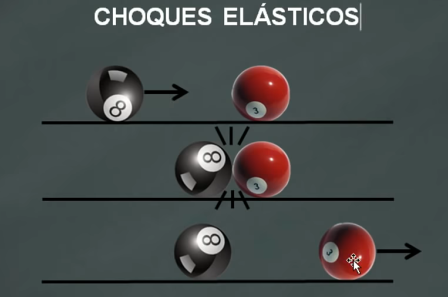
\includegraphics[width=0.7\textwidth, height=0.4\textwidth]{elastico.png}
    \caption[Colisión elástica]{Colisión elástica\footnotemark}
    \label{fig:elastico}
\end{figure}
\footnotetext{\url{https://www.youtube.com/watch?v=b9iOIr5DYj8}}


\subsubsection{Colisiones inelásticas}
Por otro lado, cuando se produce una colisión inelástica el objeto que colisiona continúa teniendo parte de la energía cinética, otra parte se transfiere al objeto que ha sido colisionado y la parte restante se disipa en forma de calor. En este tipo de choques el efecto visual es que tanto el objeto que colisiona como el objeto colisionado avanzan a cierta velocidad tras el choque. La Figura \ref{fig:inelastico} muestra un ejemplo de colisión inelástica.

\begin{figure}[h!]
    \centering
    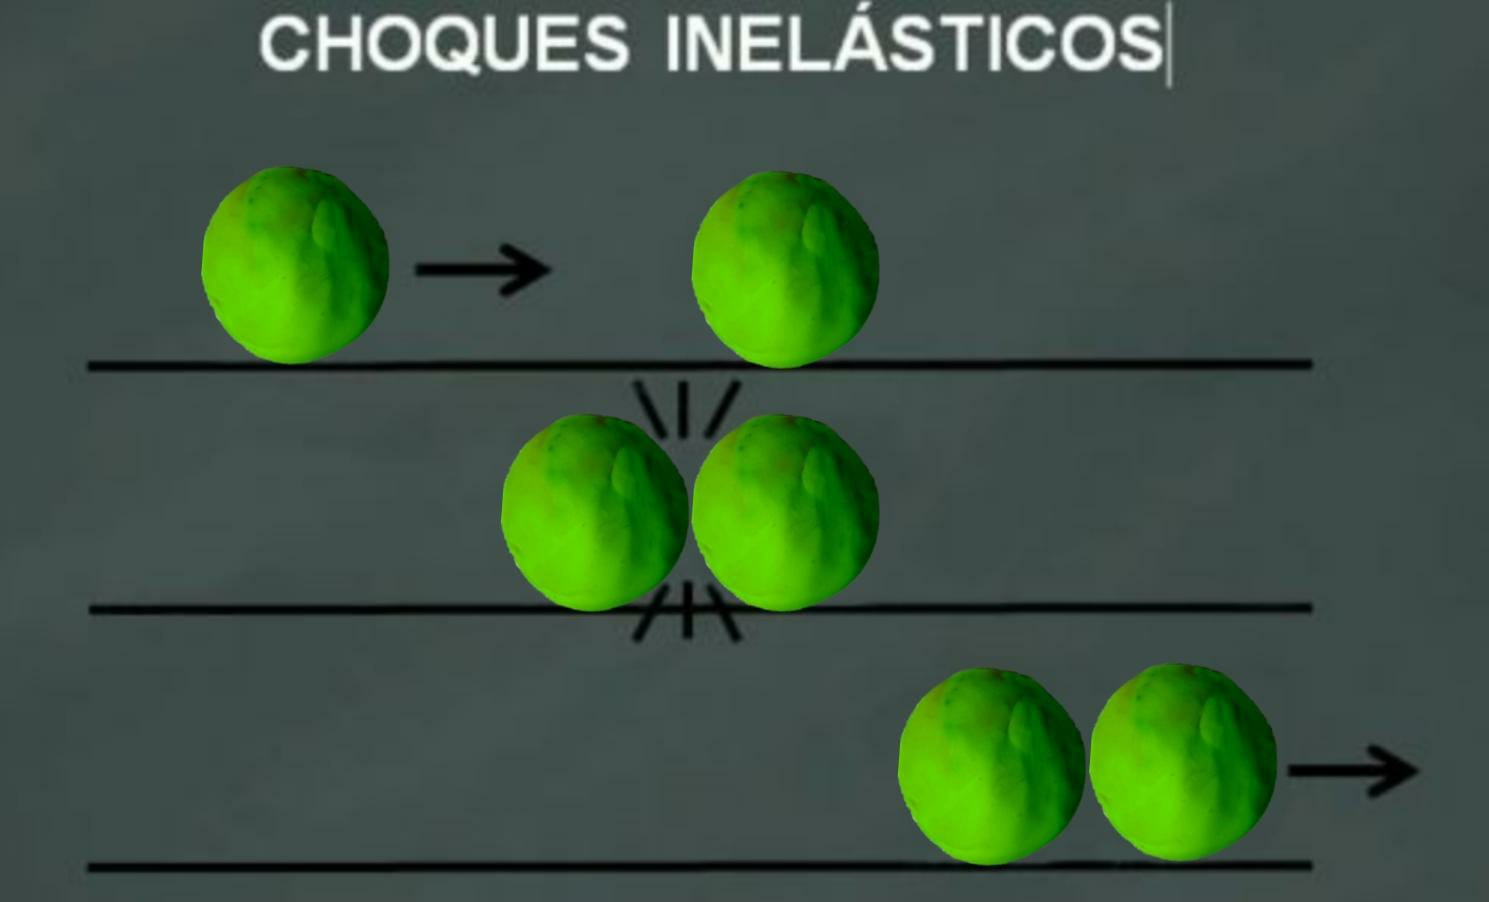
\includegraphics[width=0.7\textwidth, height=0.4\textwidth]{colision_inelastica.jpg}
    \caption[Colisión inelástica]{Colisión inelástica\footnotemark}
    \label{fig:inelastico}
\end{figure}
\footnotetext{Elaboración propia.}

\subsubsection{Pruebas de colisiones}
Se han realizado pruebas de colisiones de \textit{A-Frame} en tres escenarios diferentes variando el valor del coeficiente de restitución y la masa de los objetos. Los escenarios utilizados han sido los siguientes:

\begin{itemize}
    \item \textbf{Escenario 1:} dos pelotas cayendo por sendas rampas.
    \item \textbf{Escenario 2:} una pelota fija en el suelo y otra cayendo por una rampa.
    \item \textbf{Escenario 3:} una pelota cae por una rampa y colisiona con una pared.
\end{itemize}

\begin{figure}[!h]
  \begin{subfigure}[b]{0.3\textwidth}
    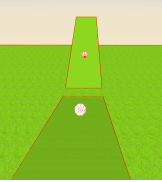
\includegraphics[width=\textwidth, height=\textwidth]{colision1.png}
    \caption{Escenario 1}
  \end{subfigure}
  \hfill
  \begin{subfigure}[b]{0.3\textwidth}
    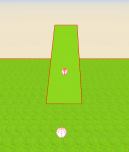
\includegraphics[width=\textwidth, height=\textwidth]{colision2.png}
    \caption{Escenario 2}
  \end{subfigure}
    \hfill
  \begin{subfigure}[b]{0.3\textwidth}
    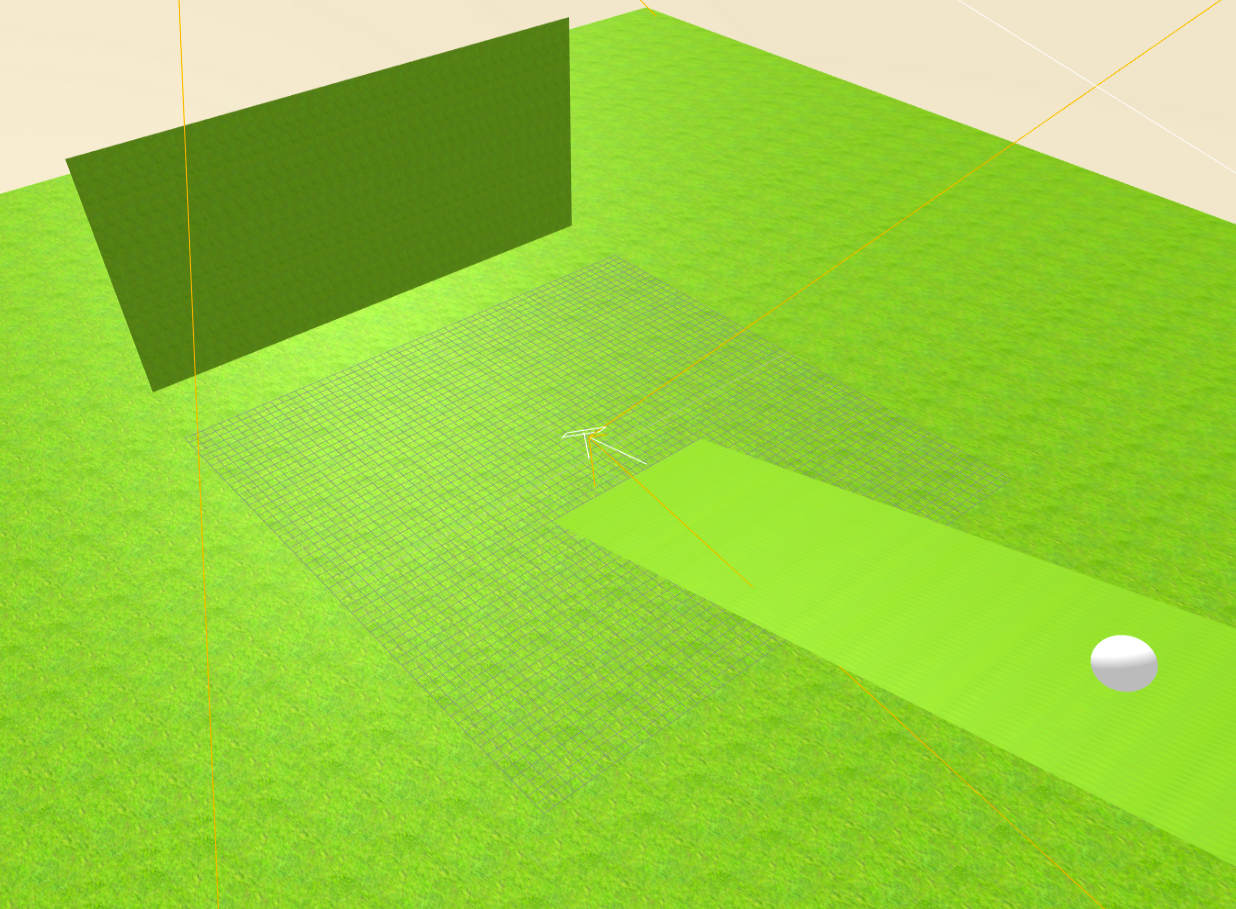
\includegraphics[width=\textwidth, height=\textwidth]{colision3.png}
    \caption{Escenario 3}
  \end{subfigure}
  \caption{Escenarios de prueba de las colisiones de \textit{A-Frame}}
 \end{figure}

Los resultados obtenidos durante las pruebas se detallan en los Cuadros \ref{fig:col-escenario1}, \ref{fig:col-escenario2} y \ref{fig:col-escenario3}. En este link\footnote{\url{https://youtu.be/T214FNFxehs}} se ofrece un vídeo con los resultados de las pruebas realizadas en el tercer escenario.
\begin{table}[]
\centering
 \resizebox{1.1\textwidth}{!}{  
\begin{tabular}{cc}
\hline
\multicolumn{1}{|c|}{\textbf{}}                 & \multicolumn{1}{c|}{\textbf{Misma masa}}                                                                                                                                    \\ \hline
\multicolumn{1}{|c|}{\textbf{Restitution = 0}}   & \multicolumn{1}{c|}{No hay rebote}                                                                                                                  \\ \hline
\multicolumn{1}{|c|}{\textbf{Restitution = 0.4}} & \multicolumn{1}{c|}{Sí hay rebote}                                                                         \\ \hline
\multicolumn{1}{|c|}{\textbf{Restitution = 1}}   & \multicolumn{1}{c|}{La pelota rebota al entrar en contacto con cualquier superfice de la escena}                                                                           \\ \hline
\multicolumn{1}{l}{}                            & \multicolumn{1}{l}{}                                                                                                                                                        \\ \hline
\multicolumn{1}{|l|}{}                          & \multicolumn{1}{c|}{\textbf{Diferente masa}}                                                                                                                                \\ \hline
\multicolumn{1}{|c|}{\textbf{Restitution = 0}}   & \multicolumn{1}{c|}{Las dos pelotas avanzan pegadas en la dirección de la de mayor masa}                                                                                    \\ \hline
\multicolumn{1}{|c|}{\textbf{Restitution = 0.4}} & \multicolumn{1}{c|}{La pelota más pesada hace cambiar la dirección del movimiento de la más ligera, que se desplaza a mayor velocidad} \\ \hline
\multicolumn{1}{|c|}{\textbf{Restitution = 1}}   & \multicolumn{1}{c|}{Las dos pelotas avanzan separadas en la dirección de la de mayor masa. La pelota de menor masa coge mayor velocidad}                                    \\ \hline
\end{tabular}
}
\caption{Resultados de las colisiones obtenidos con el escenario 1}
\label{fig:col-escenario1}
\end{table}

                                                                                                   
\begin{table}[]
\centering
 \resizebox{1.1\textwidth}{!}{  
\begin{tabular}{cc}
\hline
\multicolumn{1}{|c|}{\textbf{}}                 & \multicolumn{1}{c|}{\textbf{Misma masa}}                                                                                                                                                                                                                                                                                                                                                                               \\ \hline
\multicolumn{1}{|c|}{\textbf{Restitution = 0}}   & \multicolumn{1}{c|}{Ambas pelotas avanzan pegadas a la misma velocidad}                                                                                                                                                                                                                                                                              \\ \hline
\multicolumn{1}{|c|}{\textbf{Restitution = 0.4}} & \multicolumn{1}{c|}{La pelota que permanecía en el suelo se mueve más rápido que la que cayó por la rampa. No avanzan pegadas}                                                                                                                                                                                                                                                                           \\ \hline
\multicolumn{1}{|c|}{\textbf{Restitution = 1}}   & \multicolumn{1}{c|}{La pelota rebota al entrar en contacto con cualquier superfice de la escena}                                                                                                                                                                                                                                                                                                                      \\ \hline
\multicolumn{1}{l}{}                            & \multicolumn{1}{l}{}                                                                                                                                                                                                                                                                                                                                                                                                   \\ \hline
\multicolumn{1}{|l|}{}                          & \multicolumn{1}{c|}{\textbf{Diferente masa}}                                                                                                                                                                                                                                                                                                                                                                           \\ \hline
\multicolumn{1}{|c|}{\textbf{Restitution = 0}}   & \multicolumn{1}{l|}{\begin{tabular}[c]{@{}l@{}}- Masa pelota rampa $<$Masa pelota suelo: ambas pelotas se quedan juntas y paradas\\ - Masa pelota rampa $>$ Masa pelota suelo: ambas pelotas avanzan hacia adelante juntas y a la misma velocidad\end{tabular}}                                                        \\ \hline
\multicolumn{1}{|c|}{\textbf{Restitution = 0.4}} & \multicolumn{1}{l|}{\begin{tabular}[c]{@{}l@{}}- Masa pelota rampa $<$ Masa pelota suelo: la pelota que ha caído por la rampa rebota hacia arriba\\ - Masa pelota rampa $>$ Masa pelota suelo: la pelota que estaba en reposo avanza con más velocidad \\ que la que cayó por la rampa\end{tabular}} \\ \hline
\multicolumn{1}{|c|}{\textbf{Restitution = 1}}   & \multicolumn{1}{c|}{La pelota rebota al entrar en contacto con cualquier superfice de la escena}                                                                                                                                                                                                                                                                                                                      \\ \hline
\end{tabular}
}
\caption{Resultados de las colisiones obtenidos con el escenario 2}
\label{fig:col-escenario2}
\end{table}

\begin{table}[]
\centering
 \resizebox{1.1\textwidth}{!}{  
\begin{tabular}{cc}
\hline
\multicolumn{1}{|c|}{\textbf{}}                 & \multicolumn{1}{c|}{\textbf{Pelota con masa grande}}                                                                                       \\ \hline
\multicolumn{1}{|c|}{\textbf{Restitution = 0}}   & \multicolumn{1}{c|}{Permanece junto a la pared, sin rebote} \\ \hline
\multicolumn{1}{|c|}{\textbf{Restitution = 0.4}} & \multicolumn{1}{c|}{Sí hay rebote}                                                                       \\ \hline
\multicolumn{1}{|c|}{\textbf{Restitution = 1}}   & \multicolumn{1}{c|}{El rebote es muy elevado y vuelve a subir la rampa pŕacticamente a la misma velocidad que la bajó}         \\ \hline
                                                &                                                                                                                                \\ \hline
\multicolumn{1}{|c|}{}                          & \multicolumn{1}{c|}{\textbf{Pelota con masa pequeña}}                                                                                   \\ \hline
\multicolumn{1}{|c|}{\textbf{Restitution = 0}}   & \multicolumn{1}{c|}{Permanece junto a la pared, sin rebote}                                                                            \\ \hline
\multicolumn{1}{|c|}{\textbf{Restitution = 0.4}} & \multicolumn{1}{c|}{Cuanto más pequeña es la masa, más grande es el rebote}                                                                            \\ \hline
\multicolumn{1}{|c|}{\textbf{Restitution = 1}}   & \multicolumn{1}{c|}{Cuanto más pequeña es la masa, más grande es el rebote}                                                                            \\ \hline
\end{tabular}
}
\caption{Resultados de las colisiones obtenidos con el escenario 3}
\label{fig:col-escenario3}
\end{table}

 
\subsection{Fricción}
Cualquier cuerpo dinámico de una escena de \textit{A-Frame} presenta una fuerza de rozamiento que se opone al movimiento. Existen dos tipos de rozamiento: el rozamiento estático y el rozamiento dinámico. \textit{A-Frame} incluye tres parámetros diferentes que permiten variar el rozamiento de una superficie. No obstante, no se puede seleccionar un valor concreto para la fuerza de rozamiento estática y dinámica, ya que el atributo \textit{friction} hace variar los dos tipos de rozamiento en conjunto. Por tanto, se puede incrementar o disminuir tanto el rozamiento estático como el dinámico, pero no se pueden parametrizar con un valor concreto. \newline

Los ficheros de configuración de los escenarios de los ejercicios en formato \textit{JSON} incluyen al principio del código las siguientes líneas que permiten seleccionar el valor deseado para los atributos \textit{friction} (rozamiento estático y dinámico) y \textit{linear-damping y angular-damping} (rozamiento dinámico).

\small
\begin{verbatim}
                    "scene": {
                        "physics": "friction: 0.5"
                    }
                    attr": {
                        "static-body": {
                        "linearDamping":1.2,
                        "angularDamping":1.2
                    }
\end{verbatim}

\normalsize
\subsubsection{Rozamiento estático}
Dos superficies rígidas en reposo no se desplazan una respecto a la otra y cuando la fuerza paralela al plano tangente es suficientemente pequeña. Cuando el coeficiente de rozamiento estático de una superifice es excesivamente pequeño, los objetos que se encuentran sobre esa superficie sí se mueven con más facilidad. Una forma de calcular el coeficiente de rozamiento estático es hacer variar la inclinación de una rampa. Cuando se alcanza un ángulo de inclinación con el cual el cuerpo comienza a descender, se dice que se ha llegado al ańgulo critico. A partir del ángulo crítico se puede obtener el coeficiente de rozamiento estático gracias a la siguiente igualdad:

\begin{equation}
    tan(angulo \,\, crítico) = coeficiente \,\, de \,\, rozamiento \,\, estático \,\,
\end{equation}

\subsubsection{Rozamiento dinámico}
Cuando dos superficies están en contacto, el movimiento de una respecto a la otra genera fuerzas tangenciales llamadas fuerzas de fricción o rozamiento, las cuales tienen sentido opuesto al movimiento. La magnitud de esta fuerza depende del coeficiente de rozamiento dinámico. En \textit{A-Frame}, el rozamiento dinámico se puede configurar utilizando los atributos \textit{linear-damping y angular-damping} a nivel de objeto, además del atributo \textit{friction} a nivel de escena, como se ha mencionado anteriormente. 



\subsubsection{Pruebas de la fricción}
Se han realizado diferentes pruebas de fricción colocando un objeto en una rampa y variando la inclinación de la misma. Los resultados obtenidos han sido los siguientes:
\begin{itemize}
    \item \textbf{Prueba del rozamiento estático: } se coloca un objeto sobre una rampa y se procede a la variación de la inclinación de la misma. El objeto permanece en la misma posición hasta que se alcanza un ángulo de inclinación tan elevado que el cuerpo comienza a descender (ángulo crítico). Si se configura el atributo \textit{friction} con un valor más elevado, el ángulo crítico se alcanza más tarde, es decir, es mayor.
    \item \textbf{Prueba del rozamiento dinámico: } se mantiene fija la inclinación de la rampa y se varía el valor de los atributos \textit{friction, linear-damping y angular-damping}. Con unos valores elevados de esos tres parámetros, los robots no son capaces de subir la rampa. Sin embargo, a medida que se va reduciendo el valor de los atributos los robots comienzan a poder subir la rampa y cada vez lo hacen con mayor facilidad.
\end{itemize}

\section{Motor de físicas actual para robots en \textit{WebSim}}
Hasta el momento, \textit{WebSim} contaba con un motor de físicas completo. El movimiento de los robots se recreaba mediante la actualización de la posición cada 50 ms en función de la velocidad y la rotación consignada por el usuario. No entraban en juego aceleraciones ni fuerzas. Además, el hecho de actualizar la posición y la velocidad del robot constantemente (la velocidad se tomaba de manera instantánea de la última enviada por el cerebro software del robot. No existía diferencia entre la velocidad real y la velocidad deseada. Se asumía aceleración infinita del robot) sobreescribía encima de los cambios que introducía \textit{CANNON}, por lo que las físicas no incluían el efecto de la gravedad, la fricción ni el coeficiente de restitución. \newline 

La actualización de la posición de los robots en función de la velocidad y rotación comandadas se realizaba mediante la función \textit{updatePosition}.

\small{
\begin{verbatim} 

    updatePosition(rotation, velocity, robotPos) {
        if(simEnabled){
            let x = velocity.x / 10 * Math.cos(rotation.y * Math.PI / 180);
            let z = velocity.x / 10 * Math.sin(-rotation.y * Math.PI / 180);
            let y = (velocity.y / 10);
            robotPos.x += x;
            robotPos.z += z;
            robotPos.y += y;
        }
        return robotPos;
}
\end{verbatim}
}

\normalsize
La motivación de crear un motor de físicas complementario es que las físicas implementadas no recreaban un movimiento realista y no eran suficientes para lo que se tiene disponible en un robot real. Por ejemplo, los robots reales terrestres tienen que superar la fuerza de rozamiento para poder subir una rampa o los drones deben ser capaces de ejercer la fuerza necesaria para superar la gravedad y emprender el vuelo. Con un motor de físicas realistas, las soluciones implementadas en el simulador serán igualmente válidas para un robot físico y, además, permite la creación de ejercicios mucho más diversos, como una pista de hielo (en los que la fricción es extremadamente baja), arena (en los que la fricción es mucho más elevada) o escenarios multinivel con rampas (en los que los robots deberán ejercer fuerzas más grandes que en la superficie plana para poder ascender por la rampa). \newline

Las implicaciones que tiene la materialización de la gravedad y de la fricción son las siguientes:

\begin{itemize}
    \item \textbf{Materizalización de la gravedad:} los drones son capaces de volar en un mundo que materialice una gravedad de -9.8. Hasta el momento, los ejercicios de drones se configuraban con gravedad 0 para permitir volar al cuerpo.
    \item \textbf{Materialización de la fricción:} el desplazamiento de los robots no se realiza por imposición de una posición concreta, sino por la aplicación de la fuerza necesaria para alcanzar la velocidad objetivo. Al tener en cuenta la fricción, un robot deberá ejercer más fuerza sobre superficies con altas fricciones y menos fuerza en superficies con fricciones más pequeñas.
\end{itemize}

\clearpage
\section{Nuevo motor de físicas complementario}
\subsection{Diseño}
Este motor de físicas se utiliza para controlar el movimiento de los cuerpos dinámicos en la escena. Se le denomina complementario puesto que sólo se encarga de aplicar la fuerza autónoma al robot, dejando como tarea de \textit{CANNON} materializar las fuerzas de la fricción y la gravedad.

\begin{verbatim}
Fuerza robot = Fuerza autónoma + Fuerza gravedad + Fuerza fricción
\end{verbatim}

\begin{itemize}
    \item \underline{Fuerza gravedad:} materializada por \textit{CANNON} a un ritmo marcado por el propio motor \textit{CANNON}.
    \item \underline{Fuerza fricción:} materializada por \textit{CANNON} a un ritmo marcado por el propio motor \textit{CANNON}.
    \item \underline{Fuerza autónoma:} lo materializa nuestro motor complementario a su propio ritmo (distinto del de Cannon) y teniendo en cuenta las velocidades deseadas que marca en cada instante el código fuente del cerebro programado. El ritmo que se ha fijado ha sido de 20 ms.
\end{itemize}

Esta idea de motor complementario es radicalmente distinta de la implementación que existía hasta el momento. La función \textit{updatePosition} actúaba como un motor completo que sobreescribía a \textit{CANNON}. No existía combinación alguna entre ambos motores. \newline


La arquitectura del motor de físicas complementario presenta dos niveles. El nivel superior conecta directamente con el cerebro software del robot, el cual es capaz de dar continuamente instrucciones en posición y en velocidad. No obstante, ambos tipos de instrucciones se basan en comandar una velocidad objetivo. En el caso de las instrucciones en posición el robot se moverá a la velocidad objetivo hasta que se alcance la posición consignada en la instrucción y en el caso de las instrucciones en velocidad, el movimiento no termina. Este nivel más alto se basa en un controlador PD que traduce las consignas de velocidad que le llegan del cerebro, en la fuerza necesaria a aplicar al robot para alcanzar dichas velocidades consignadas. Estas fuerzas son las que entiende el núcleo o nivel más bajo del motor de físicas. Conociendo la masa y el momento de incercia, las fuerzas obtenidas se podrán traducir en aceleraciones. La Figura \ref{fig:motor_diseño} muestra un esquema del diseño del motor. \newline

Por otro lado, se incluye la tabla \ref{fig:parametros} que introduce a modo de resumen todos los parámetros que caraceterizan el movimiento
de los robots autónomos con el nuevo motor de físicas complementario. Tanto parámetros del modelo de fuerzas (masa, momento de inercia, fuerza máxima, torque máximo, maxima velocidad lineal, maxima velocidad angular, máxima aceleración lineal y máxima aceleración angular) como parámetros de \textit{A-Frame} (coeficiente de restitución, gravedad, fricción, amortiguación lineal y amortiguación angular). Los últimos ya se han explicado y los primeros se describen a continuación.

\begin{figure}[h!]
    \centering
    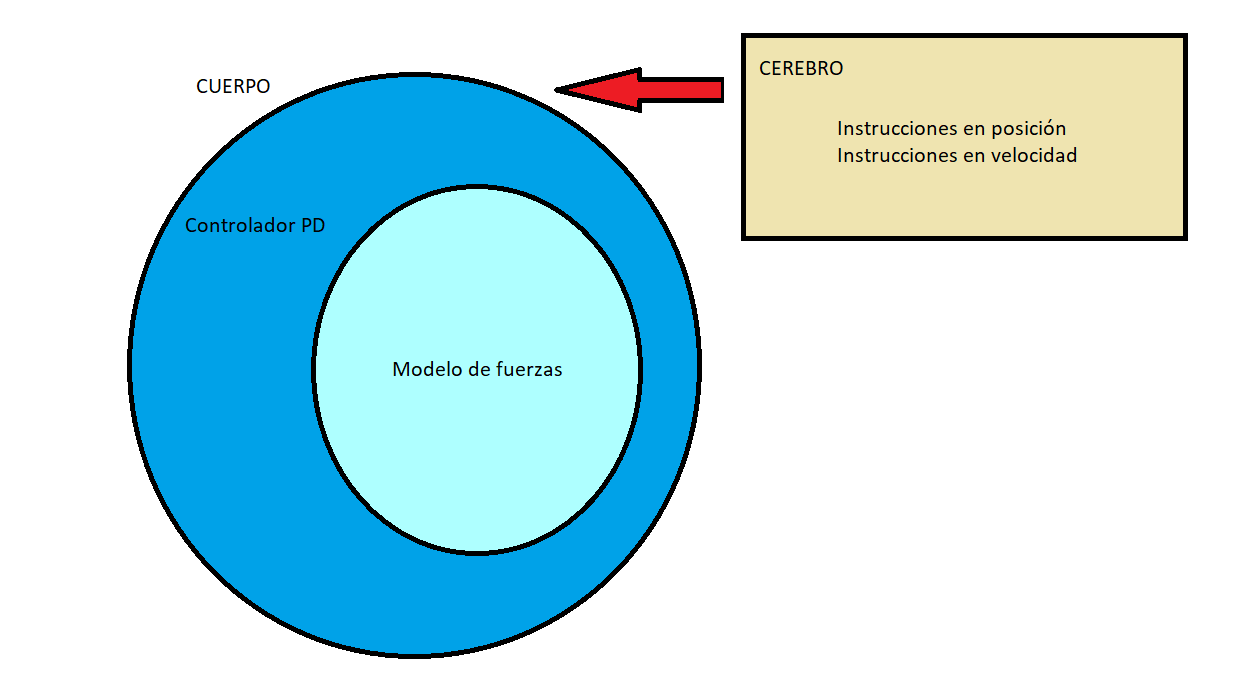
\includegraphics[scale=0.8]{Diseño_motor_4.PNG}
    \caption[Diseño del motor de físicas complementario]{Diseño del motor de físicas complementario\footnotemark}
    \label{fig:motor_diseño}
\end{figure}
\footnotetext{Elaboración propia.}

\begin{table}[h!]
\centering
\resizebox{15cm}{!}{
\begin{tabular}{|c|c|}
\hline
\multicolumn{2}{|c|}{\textbf{Parámetros del modelo de fuerzas}}                                                                          \\ \hline
mass                   & Masa del robot                                                                                                  \\ \hline
inertia                & Momento de inercia del robot                                                                                    \\ \hline
Fmax                   & Fuerza máxima aplicable                                                                                         \\ \hline
Tmax                   & Torque máximo aplicable                                                                                         \\ \hline
accelerationMax        & Aceleración lineal máxima                                                                                       \\ \hline
angularAccelerationMax & Aceleración angular máxima                                                                                      \\ \hline
linealSpeedMax         & \begin{tabular}[c]{@{}c@{}}Velocidad lineal máxima \\ que puede alcanzar el robot\end{tabular}                  \\ \hline
angularSpeedMax        & \begin{tabular}[c]{@{}c@{}}Velocidad angular máxima \\ que puede alcanzar el robot\end{tabular}                 \\ \hline
\multicolumn{2}{|c|}{\textbf{Parámetros de \textit{A-Frame}}}                                                           \\ \hline
restitution            & \begin{tabular}[c]{@{}c@{}}Conservación de la energía cinética \\ \\ en un choque entre partículas\end{tabular} \\ \hline
gravity                & Gravedad                                                                                                        \\ \hline
friction               & Fricción (rozamiento estático y dinámico)                                                                       \\ \hline
linearDamping          & \begin{tabular}[c]{@{}c@{}}Amortiguación lineal \\ (rozamiento dinámico en el movimiento lineal)\end{tabular}   \\ \hline
angularDamping         & \begin{tabular}[c]{@{}c@{}}Amortiguación angular \\ (rozamiento dinámico en el movimiento angular)\end{tabular} \\ \hline
\end{tabular}
}
\caption{Parámetros que caracterizan el movimiento de un robot autónomo}
\label{fig:parametros}
\end{table}

\clearpage
\subsection{Modelo de fuerzas}
El núcleo del nuevo motor de físicas es un modelo de fuerzas en el que, a partir de la definición de la masa y el momento de inercia del robot, se calcula la aceleración o torque a aplicar. De esta manera, un robot muy pesado deberá ejercer una fuerza mayor que un robot más ligero para alcanzar una misma velocidad. \newline

Para que el modelo funcione es necesaria la definición de los siguientes parámetros:
\begin{itemize}
    \item \textbf{Fuerza máxima:} es la fuerza autónoma máxima que puede aplicar un robot. Concede realismo al modelo, puesto que termina con la asunción de aceleración infinita.
    \item \textbf{Torque máximo:} es el momento autónomo de fuerza máximo que puede aplicar un robot, es decir, es la fuerza máxima de giro aplicable. Concede realismo al modelo, puesto que termina con la asunción de aceleración infinita.
    \item \textbf{Velocidad lineal máxima:} es la velocidad lineal máxima que puede alcanzar un robot.
    \item \textbf{Velocidad angular máxima:} es la velocidad angular máxima que puede alcanzar un robot.
    \item \textbf{Masa:} es necesaria para obtener el valor de la aceleración lineal.
    \item \textbf{Momento de inercia:} es la medida de la inercia rotacional cuando un cuerpo gira. Es el equivalente a la masa en un movimiento angular. Es necesario para obtener el valor de la aceleración angular.
\end{itemize}

\small
\begin{verbatim}

                /* Masa e incercia*/
                const mass = this.robot.body.mass;
                const inertia = this.robot.body.inertia.x;
                
                /* Fuerza y torque máximos */
                const fMax = 100;
                const tMax = 100;
                    
                    
                    
                /* Aceleración lineal y angular máxima */
                const accelerationMax = fMax / mass;
                const angularAccelerationMax = tMax / inertia;
                
                /* Aceleración lineal y angular máxima */
                const linearSpeedMax = 10;
                const angularSpeedMax= 5; 
                
                
\end{verbatim}



\subsection{Controlador PD}
\normalsize
El controlador PD se encarga de la traducción de las velocidades deseadas que le llegan al motor complementario en cada momento del cerebro a la fuerza autónoma a aplicar al robot. \newline

El controlador PD es una variante del controlador PID (controlador proporcional, integral y derivativo) que no incluye la componente integral. Se trata de un controlador por realimentación que calcula la desviación o error entre una medida y el valor que se desea obtener. Cada componente tiene una utilidad diferente y depende de distintos factores:
\begin{itemize}
    \item \textbf{Componente proporcional: }depende del error actual y su función es minimizar el error del sistema.
    \item \textbf{Componente derivativa: }depende de los errores pasados y permite estabilizar el sistema reduciendo la oscilación del valor de salida.
    \item \textbf{Componente integral: }es una predicción de los errores futuros y se utiliza cuando el componente derivativo no consigue reducir el error del sistema. Su uso es complejo ya que puede producir la desastibilización del sistema.
\end{itemize}

\clearpage
\begin{figure}[h!]
    \centering
    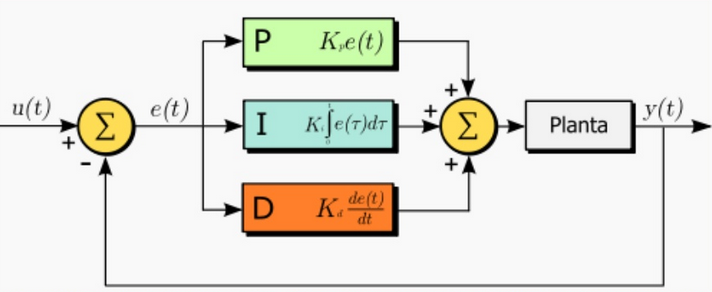
\includegraphics[scale=0.7]{pid.png}
    \caption[Controlador PID]{Controlador PID \footnotemark}
    \label{fig:pid}
\end{figure}
\footnotetext{https://es.slideshare.net/quasar.0360.7912/sintonizacion-de-controladores-pid}

Mediante un sencillo algoritmo basado en la suma de estos tres componentes, el controlador es capaz de ajustar su salida a un valor de referencia. Además, el modelo incluye tres constantes que se emplean para ponderar los componentes anteriores. En este caso sólo se van a tener en cuenta los componentes proporcionales y derivativos puesto que se van a implementar controladores PD  porque el error del sistema no es excesivamente elevado.\newline 

\begin{figure}[h!]
    \centering
    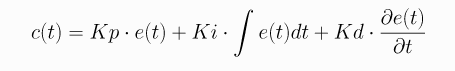
\includegraphics[scale=0.5]{pid_form.png}
    \label{fig:pid_form}
\end{figure}

Esta capa del motor incluye cuatro controladores PD diferentes que se ejecutan dependiendo del tipo de robot que esté realizando el movimiento (robot terrestre o drone) y del tipo de movimiento que se efectúe (avance lineal, giro, vuelo o suspensión en el aire). A continuación, se detallan los cuatro tipos de controladores incluidos.

\begin{itemize}
    \item \textbf{Controlador PD en velocidad del plano horizontal:} además de la velocidad horizontal deseada, coge como entrada la velocidad resultante del plano horizontal en ese instante y genera como salida la fuerza que debe ejercer el robot para alcanzar la velocidad objetivo. 
    
    \begin{figure}[h!]
    \centering
    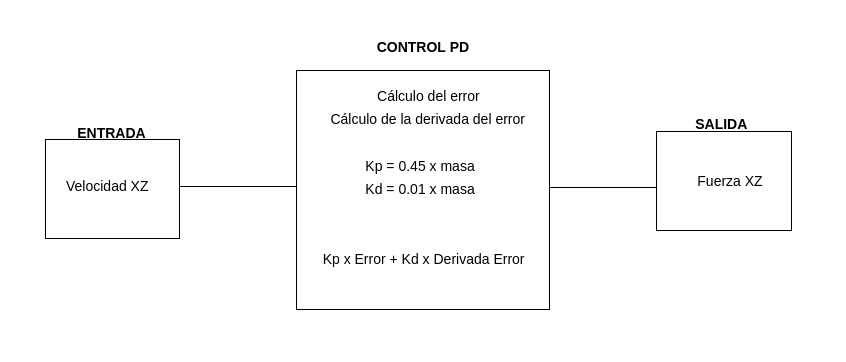
\includegraphics[width=\textwidth, height=0.4\textwidth]{controlador_PD_XZ.png}
    \caption[Diseño controlador PD en velocidad del plano horizontal]{Diseño controlador PD en velocidad del plano horizontal\footnotemark}
    \label{fig:esquema_pd_1}
    \end{figure}
    \footnotetext{Elaboración propia.}
    
    \item \textbf{Controlador PD en velocidad del eje vertical:} además de la velocidad vertical deseada, coge como entrada la componente vertical de la velocidad en ese instante y genera como salida la fuerza que debe ejercer el robot para alcanzar la velocidad objetivo. 
    
    \begin{figure}[h!]
    \centering
    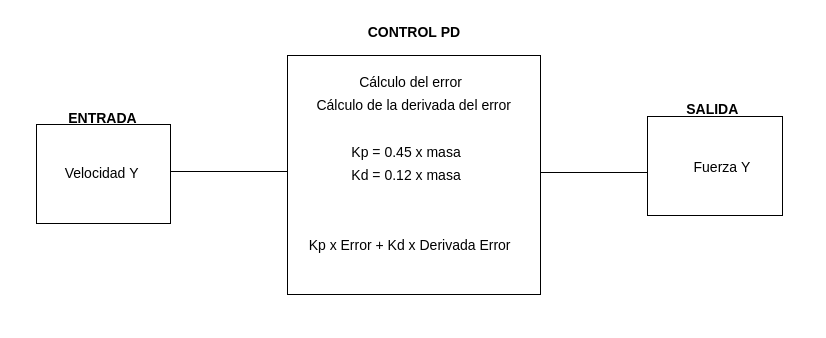
\includegraphics[width=\textwidth, height=0.4\textwidth]{controlador_PD_vel_Y.png}
\caption[Diseño controlador PD en velocidad del eje vertical]{Diseño controlador PD en velocidad del eje vertical\footnotemark}
    \label{fig:esquema_pd_2}
    \end{figure}
    \footnotetext{Elaboración propia.}
    
    \item \textbf{Controlador PD en velocidad angular horizontal (yaw):} además de la velocidad deseada de guiñada, coge como entrada la velocidad angular en ese instante y genera como salida el torque que debe ejercer el robot para alcanzar la velocidad de giro objetivo. 
    
    \clearpage
    \begin{figure}[h!]
    \centering
    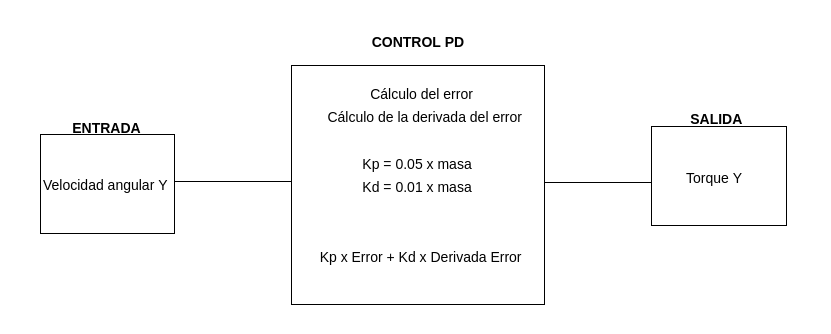
\includegraphics[width=\textwidth, height=0.4\textwidth]{control_PD_angular_drone.png}
\caption[Diseño controlador PD en velocidad angular horizontal para drone]{Diseño controlador PD en velocidad angular horizontal para drone\footnotemark}
    \label{fig:esquema_pd_3}
    \end{figure}
    \footnotetext{Elaboración propia.}

    \begin{figure}[h!]
    \centering
    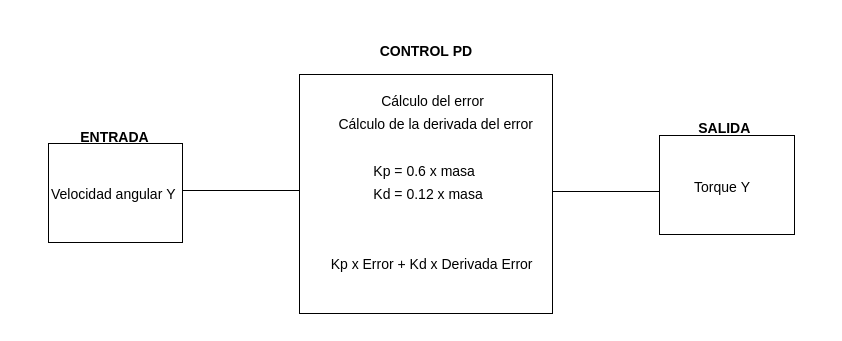
\includegraphics[width=\textwidth, height=0.4\textwidth]{control_PD_angular_tierra.png}
\caption[Diseño controlador PD en velocidad angular horizontal para robot terrestre]{Diseño controlador PD en velocidad angular horizontal para robot terrestre\footnotemark}
    \label{fig:esquema_pd_4}
    \end{figure} 
    \footnotetext{Elaboración propia.}
    
    \item \textbf{Controlador PD en posición para la altura:} coge como entrada la componente vertical de la posición en ese instante y genera como salida la fuerza que debe ejercer el robot para mantener una posición de referencia. Se usa cuando la velocidad deseada es cero. El control en velocidad vertical cuando la velocidad consignada es cero tiembla un poco, haciendo que el movimiento del drone pierda realismo. Por esta razón, se ha optado por materializar esa velocidad vertical cero con el control en posición vertical, con el que se obtiene un mejor resultado.
    
    \clearpage
    \begin{figure}[h!]
    \centering
    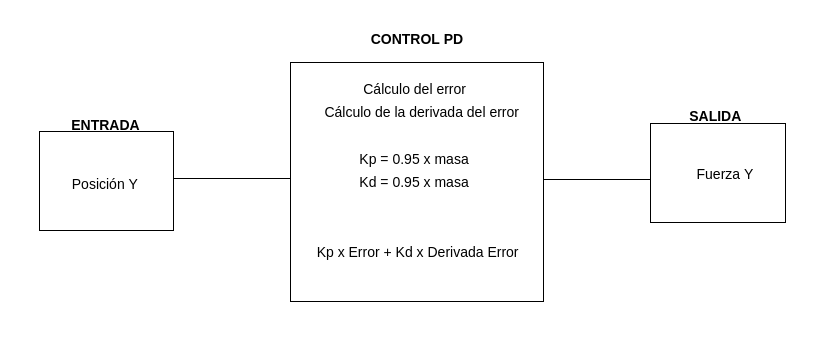
\includegraphics[width=\textwidth, height=0.4\textwidth]{controlador_PD_pos_Y.png}
    \caption[Diseño controlador PD en posición para la altura]{Diseño controlador PD en posición para la altura\footnotemark}
    \label{fig:esquema_pd_5}
    \end{figure}
    \footnotetext{Elaboración propia.}
\end{itemize}

De los controladores PD implementados, son específicos para el funcionamiento del drone el controlador PD en velocidad del eje vertical (empleado en el vuelo) y el controlador PD en posición para la altura (necesario cuando el robot debe permanecer inmóvil durante el vuelo en una posición concreta). El controlador PD en velocidad del plano horizontal es empleado en el movimiento lineal tanto de robots terrestres como de drones y el controlador PD en velocidad angular horizontal se utiliza durante los giros tanto de robots terrestres como de drones. No obstante, las constantes proporcional y derivativa y el torque máximo varían en función del tipo de robot, puesto que en el caso del drone la fricción no opone resistencia durante el giro, ya que este se encuentra volando sin mantener contacto con ninguna superficie.
    
\normalsize
\subsection{Timing}
Este concepto es de especial relevancia ya que es el que hace que el motor sea complementario y no completo, es decir, es lo que permite que el motor complementario se combine satisfactoriamente con el de \textit{CANNON} y no sobreescriba sus modificaciones. \newline

El motor de físicas complementario se ejecuta cada 20 ms gracias a un \textit{timeout} que lo invoca de forma periódica. Pero, ¿cuándo se ejecuta el motor de \textit{CANNON}? 

\small {
\begin{verbatim}
            setTimeout(this.auxiliaryPhysics.bind(this), 20);
\end{verbatim}
}

\normalsize
\textit{CANNON} actualiza sus físicas en cada iteración del bucle de renderizado de \textit{A-Frame}. Además, no lleva una cuenta explícita del tiempo y tampoco lo tiene en cuenta a la hora de modificar las posiciones y velocidades de los objetos de la escena. Puesto que la frecuencia de ejecución de \textit{CANNON} es superior a la del motor complementario, ha sido necesario calcular el número de veces que se ejecuta el código \textit{CANNON} entre dos iteraciones del motor de físicas complementario para poder realizar una correcta combinación entre ambos. El motor complementario deberá aplicar en cada iteración una aceleración X veces superior a la que corresponde, siendo X el número de veces que ha entrado \textit{CANNON} desde la útima vez que se ejecutó el motor complementario. \newline

\small {
\begin{verbatim}
    Aceleración autónoma = iteracionesCANNON x aceleración calculada
    
\end{verbatim}
}

\normalsize
El cómputo de las iteraciones de \textit{CANNON} se ha realizado creando un nuevo componente auxiliar que hace incrementar en uno un contador por cada tick de renderizado que ejecuta \textit{A-Frame}. \newline


Las variables y funciones que se han añadido al código original para llevar a cabo la implementación se incluyen a continuación. Las funciones \textit{tickCounter, getTickCounter y setTickCounter} se han utilizado para contabilizar el número de veces que se ejecuta el motor de \textit{CANNON} entre dos iteraciones del motor complementario.

\small {
\begin{verbatim}
                export var tickCounter = 0;
                
                export function getTickCounter() {
                    return tickCounter;
                }
                export function setTickCounter(value) {
                    tickCounter = value;
                }
\end{verbatim}
}

\normalsize
Para crear el nuevo componente auxiliar se han utilizado las herramientas que ofrece \textit{A-Frame} para el registro de nuevos componentes. La siguiente línea de código realiza el registro del nuevo componente auxiliar que se utiliza para contabilizar las iteraciones de \textit{CANNON}. A continuación, también se ha incluido el código del tick del nuevo componente registrado.

\small {
\begin{verbatim}


            /* Registro del nuevo componente */
            AFRAME.registerComponent("iterations", iterationsObj);
            
            /* Función tick del componente "iterations" */
            export var iterationsObj = {
                schema: {
                  count: { type: 'number', default: 0 },
                  position: { "x":0, "y":0, "z":0}
                },
                tick: function(){
                  setTickCounter(getTickCounter() + 1);
                  console.log('Tick de renderizado de A-FRAME');
                }
              }
            }
            
            
\end{verbatim}
}

\normalsize
Gracias a la correcta combinación temporal de ambos motores, se consigue que el motor de físicas complementario calcule la fuerza autónoma a aplicar a los robots dinámicos y \textit{CANNON} materialice la gravedad y fricción de la escena. La Figura \ref{fig:combi_motor} muestra la combinación existente actualmente entre ambos motores, que permite que se hable de un motor complementario y no de un motor completo. Cada motor lleva incorporado un reloj de ejecución independiente y, en el caso de \textit{CANNON}, es necesario disponer de un contador de ticks para monitorizar su hilo de ejecución.

\clearpage
\begin{figure}[h!]
    \centering
    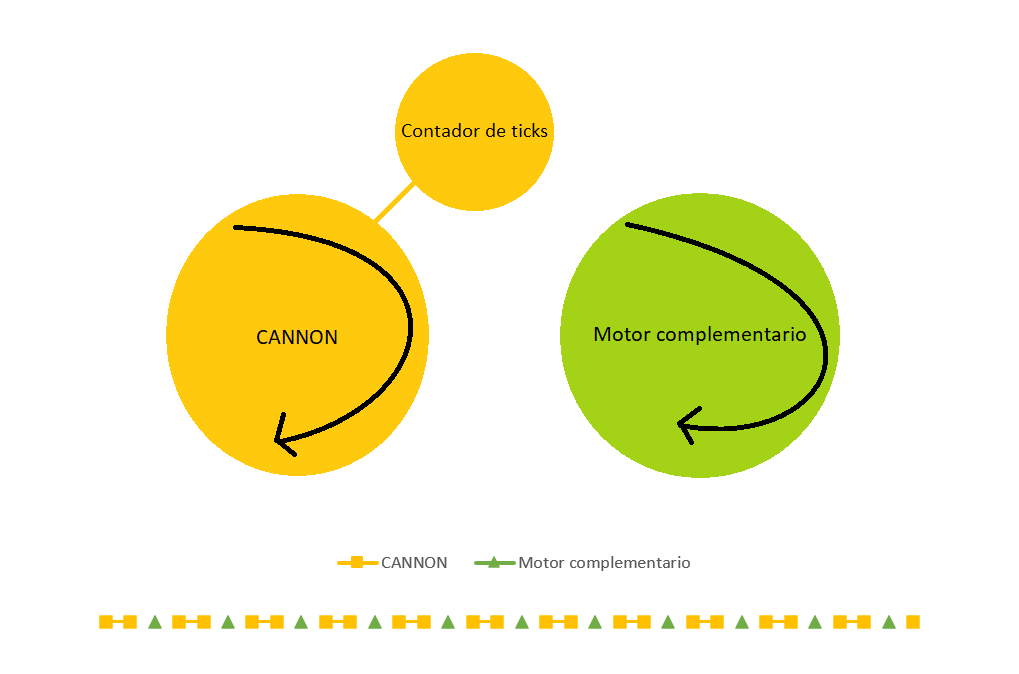
\includegraphics[scale=0.9]{combinacion_motores_2.PNG}
    \caption[Combinación de los motores de físicas a lo largo del tiempo]{Combinación de los motores de físicas a lo largo del tiempo\footnotemark}
    \label{fig:combi_motor}
\end{figure}
\footnotetext{Elaboración propia.}

\subsection{Implementación}
A continuación se incluyen los fragmentos de código que ha sido necesario incluir en el fichero \textit{interfacesRobot.js} del \textit{Simcore} de \textit{WebSim} para el correcto funcionamiento del motor complementario. \newline

\textbf{Adición de variables a la clase robot ya creada.} De esta manera, el motor complementario es escalable a ejercicios multirobot. Cada robot mantiene un registro propio del valor de sus variables.
\small {
\begin{verbatim}




                export class RobotI {
                    constructor(robotId) {
                        this.errorY = 0;
                        this.errorXZ = 0;
                        this.errorW = 0;
                        this.errorActualY = 0;
                        this.errorActualXZ = 0;
                        this.errorActualW = 0;
                        this.derivadaErrorY = 0;
                        this.derivadaErrorXZ = 0;
                        this.derivadaErrorW = 0;
                        this.forcePD = 0;
                        this.accelerationPD = 0;
                        this.commandedVelocityY = 0;
                        this.commandedVelocityXZ = 0;
                        this.commandedVelocityW = 0;
                        this.accelerationPDY = 0;
                        this.accelerationPDXZ = 0;
                        this.accelerationPDW = 0;
                        this.resultVelocity = 0;
                        this.refPos = 0;
                        this.init = true;
                        this.stop = true;
                        this.motorIterations = 0;
                }
                
                
                
                
                
                
                
                
\end{verbatim}
}

\normalsize
\textbf{Función auxiliaryPhysics.} Es la función que materializa el motor complementario y se ejecuta cada 20 ms gracias al \textit{timeout} que se ha añadido al final de la misma.

\footnotesize {
\begin{verbatim}
/*Actualización del contador de iteraciones*/
auxiliaryPhysics() {
    /* Control de velocidades máximas */
    var vmax = this.robot.getAttribute('vmax');
	var wmax = this.robot.getAttribute('wmax');
	if (this.robot.getAttribute('vmax') == null) {
	    var vmax = 10;
	}
	    
    if (this.robot.getAttribute('wmax') == null) {
        var wmax = 5;
	}
    this.motorIterations = getTickCounter(); 
               
    /* Sólo para Drone */
    /* Si la velocidad de vuelo objetivo es 0: */
    if ((this.velocity.y <= 0.0001) || (this.velocity.y <= -0.0001)){
        if (this.init == true) {
        /* Si el movimiento aún no ha comenzado la aceleración debe ser 0 */
            this.accelerationPDY = 0;
        } else { 
        /* Si el movimiento ya ha comenzado: */
    	    if (this.stop == true) {
    	/* Si se acaba de quedar en suspensión, guardo la posición de referencia */
    		  this.refPos = this.robot.body.position.y;
    		 }
    	/* Entra el controlador PD en posiciones */
            this.stop = false;
    		this.accelerationPDY = this.controladorPDVerticalPos();
    	}
    /* Si la velocidad objetivo no es 0, se ejecuta el controlador PD en velocidades */
    } else {
        this.init = false;
        this.stop = true;
        this.accelerationPDY = this.controladorPDVerticalVel();
    }
                
    /* Se utiliza la aceleración calculada con los controladores para obtener la 
    velocidad a aplicar utilizando las fórmulas MRUA y la combinación entre motores */
                
        this.commandedVelocityY = this.robot.body.velocity.y + 
        this.motorIterations*this.accelerationPDY;
        
	    if (Math.abs(this.commandedVelocityY) > vmax) {
            	if (this.commandedVelocityY > 0) {
                    this.commandedVelocityY = vmax;
            	} else {
                    this.commandedVelocityY = -vmax;
            	}
        }   
        
        this.robot.body.velocity.set(this.robot.body.velocity.x, 
        this.commandedVelocityY, this.robot.body.velocity.z); 
    }
    /* Movimiento en el plano horizontal: drone y robot terreste */
    
    /* Velocidad resultante = RaízCuadrada(Vx ² + Vz²)*/
	this.resultVelocity = Math.sqrt(Math.pow(this.robot.body.velocity.x, 2) + 
	Math.pow(this.robot.body.velocity.z, 2));
	
	/* Entra el controlador PD */
	this.accelerationPDXZ = this.controladorPDHorizontal(this.resultVelocity); 
	
	/* Se utiliza la aceleración calculada con los controladores para obtener la velocidad 
a aplicar utilizando las fórmulas MRUA y la combinación entre motores */
	this.commandedVelocityXZ = this.resultVelocity + 
	this.motorIterations*this.accelerationPDXZ;
	let rotation = this.getRotation();
	
	if (Math.abs(this.commandedVelocityXZ) > vmax) {
    	if (this.commandedVelocityXZ > 0) {
    	    this.commandedVelocityXZ = vmax;
    	} else {
    	    this.commandedVelocityXZ = -vmax;
        }
    }	
	
	/* La velocidad comandada resultante se descompone en las velocidades Vx y Vz */
	this.robot.body.velocity.set(this.commandedVelocityXZ*Math.cos(rotation.y*Math.PI/180), 
	this.robot.body.velocity.y,this.commandedVelocityXZ*Math.sin(-rotation.y*Math.PI/180));
	
    /* Movimiento angular: drone y robot terreste */
    
    /* Entra el controlador PD angular */              
    this.accelerationPDW = this.controladorPDAngular();
    
    /* Se utiliza la aceleración calculada con el controlador para obtener 
    la velocidad angular a aplicar utilizando las fórmulas MRUA y la 
    combinación entre motores */
    this.commandedVelocityW = this.robot.body.angularVelocity.y + 
    this.motorIterations*this.accelerationPDW;

    if (Math.abs(this.commandedVelocityW) > wmax) {
    	if (this.commandedVelocityW > 0) {
    	    this.commandedVelocityW = wmax;
        } else {
            this.commandedVelocityW = -wmax;
        }
    }     
    
    this.robot.body.angularVelocity.set(0, this.commandedVelocityW, 0);
    
    setTimeout(this.auxiliaryPhysics.bind(this), 20);
}





\end{verbatim}
}
\normalsize
\textbf{Controladores PD.} Se incluye como muestra del software implementado el controlador PD en velocidad del plano horizontal y el controlador PD en posición para la altura. Los controladores restantes presentan un código muy similar a estos.

\footnotesize {
\begin{verbatim}
/* Código del controlador PD en velocidad del plano horizontal */
    controladorPDHorizontal(resultVelocity) {
    /* Definición constantes para el controlador, fuerza máxima y aceleración máxima */
        const kp = 0.45;
        const kd = 0.01;
        const mass = this.robot.body.mass;
        var fMax = this.robot.getAttribute('fmax');
        if (this.robot.getAttribute('fmax') == null) {
	    	var fMax = 1000000;
	    }
        const accelerationMax = fMax / mass;

        /* Cálculo del error y derivada del error*/
        this.errorActualXZ = this.velocity.x - resultVelocity;
        this.derivadaErrorXZ = this.errorActualXZ - this.errorXZ;
        this.errorXZ = this.errorActualXZ;

        /* Salida del controlador */
        this.forcePD = kp*this.errorActualXZ + kd*this.derivadaErrorXZ;
        
        /* Obtención de la aceleración teniendo en cuenta la masa */
        this.accelerationPD = this.forcePD / mass;

        /* Límite de aceleración aplicable en cada iteración */
        if (Math.abs(this.accelerationPD) > angularAccelerationMax) {
            if (this.accelerationPD > 0) {
                this.accelerationPD = angularAccelerationMax;
            } else {
                this.accelerationPD = - angularAccelerationMax;
            }
        }
        return this.accelerationPD;
    }
\end{verbatim}
}

\footnotesize {
\begin{verbatim}  
/* Código del controlador PD en posición para la altura*/
    controladorPDVerticalPos() {
        /* Definición constantes para el controlador, fuerza máxima y                   aceleración máxima */
        const kp = 0.95;
        const kd = 0.95;
        const mass = this.robot.body.mass;
        var fMax = this.robot.getAttribute('fmax');
        if (this.robot.getAttribute('fmax') == null) {
	    	var fMax = 1000000;
	    }
        const accelerationMax = fMax / mass;
        

        /* Cálculo del error y derivada del error*/
        this.errorActualY = this.refPos - this.robot.body.position.y;
        this.derivadaErrorY = this.errorActualY - this.errorY;
        this.errorY = this.errorActualY;
        
        /* Salida del controlador */
        this.forcePD = kp*this.errorActualY + kd*this.derivadaErrorY;
        
        /* Obtención de la aceleración teniendo en cuenta la masa */
        this.accelerationPD = this.forcePD / mass;

        /* Límite de aceleración aplicable en cada iteración */
        if (Math.abs(this.accelerationPD) > angularAccelerationMax) {
            if (this.accelerationPD > 0) {
                this.accelerationPD = angularAccelerationMax;
            } else {
                this.accelerationPD = - angularAccelerationMax;
            }
        }
        return this.accelerationPD;
    }
}
\end{verbatim}
}

\normalsize
\section{Validación experimental}
\subsection{Simulación realista de robots terrestres}
El motor de físicas complementario permite dotar a \textit{WebSim} de un motor de físicas más realistas puesto que únicamente actúa sobre la fuerza autónoma del robot, dejando libertad a \textit{CANNON} para materializar tanto fricción como gravedad. Gracias a ello, se simulan mundos en los que los requisitos se asemejan en mayor medida a las características que se encuentran en el mundo real y en los robots físicos. \newline

En consecuencia, se van a poder desarrollar ejercicios más variados como pistas de hielo o ejercicios multinivel con rampas que interconecten los múltiples niveles. El modelo de físicas es ahora mucho más realista, pero hay que configurarlo adecuadamente para
cada robot eligiendo valores apropiados para sus parámetros. A continuación, se incluyen varios ejemplos en los que se puede observar cómo, con una correcta configuración de los atributos, se puede lograr la simulación de situaciones muchos más diversas y realistas:

\begin{itemize}

  \item \textbf{Fuerza máxima = 0.1.} No es posible ascender por una rampa dado que la fuerza máxima del mBot no es suficiente para superar la fricción. Esta situación puede solucionarse disminuyendo la fricción de la escena, reduciendo la inclinación de la rampa o aumentando la fuerza máxima del robot\footnote{\url{https://youtu.be/LQk9GLoMIk0}}.
    
    \begin{figure}[h!]
  \begin{subfigure}[b]{0.3\textwidth}
    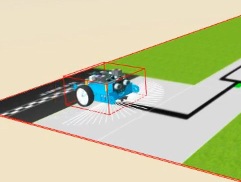
\includegraphics[width=\textwidth, height=\textwidth]{rampa1.png}
  \end{subfigure}
  \hfill
  \begin{subfigure}[b]{0.3\textwidth}
    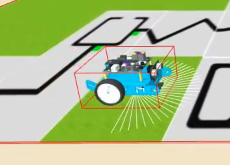
\includegraphics[width=\textwidth, height=\textwidth]{rampa 2.png}
  \end{subfigure}
    \hfill
  \begin{subfigure}[b]{0.3\textwidth}
    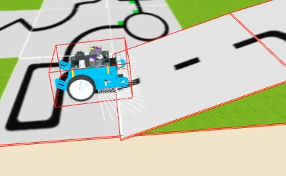
\includegraphics[width=\textwidth, height=\textwidth]{rampa3.png}
  \end{subfigure}
\caption{Subida de rampa con una fuerza máxima insuficiente}
\label{fig:rampa}
\end{figure}
    \item \textbf{Fricción = 0.00000001.} El escenario se puede asimilar a una pista de hielo. Cuando se le consigna al robot una instrucción en posición, por ejemplo 'gira 90º a la izquierda', se observa cómo el robot no es capaz de frenar el movimiento a los 90º a pesar de que su controlador PD angular comienza a comandar fuerzas para tratar de frenarlo. Sin embargo, como la fricción es excesivamente pequeña el controlador tarda más tiempo en lograr frenar el movimiento, tal y como ocurriría en una pista de hielo\footnote{\url{https://www.youtube.com/watch?v=QfPmtPeEL5k}}. La Figura \ref{fig:pistahielo} muestra la ejecución de esta instrucción y se observa cómo el robot finaliza el movimiento prácticamente a los 180º por esta razón.

\begin{figure}[h!]
  \begin{subfigure}[b]{0.5\textwidth}
    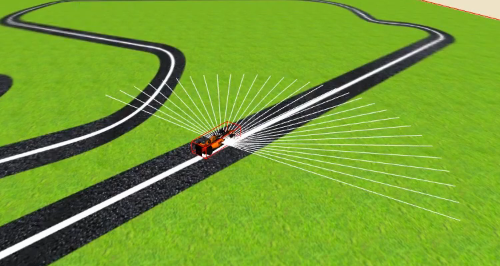
\includegraphics[width=\textwidth, height=\textwidth]{pistahielo1.png}
  \end{subfigure}
  \hfill
  \hfill
  \begin{subfigure}[b]{0.5\textwidth}
    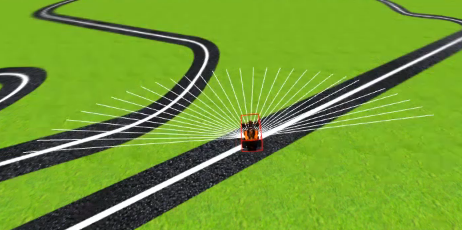
\includegraphics[width=\textwidth, height=\textwidth]{pistahielo2.png}
  \end{subfigure}
    \hfill
    \hfill
  \begin{subfigure}[b]{0.5\textwidth}
    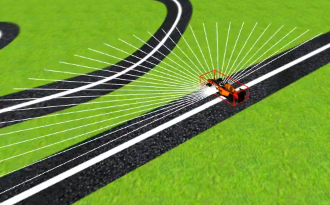
\includegraphics[width=\textwidth, height=\textwidth]{pistahielo3.png}
  \end{subfigure}
    \hfill
  \begin{subfigure}[b]{0.5\textwidth}
    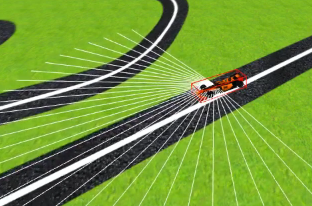
\includegraphics[width=\textwidth, height=\textwidth]{pistahielo4.png}
  \end{subfigure}
\caption{Giro de 90º hacia la izquierda en una superficie con una fricción muy baja}
\label{fig:pistahielo}
\end{figure}
\end{itemize}

La Figura \ref{fig:friccion-acele} muestra cómo influye en la aceleración autónoma que aplica el motor de físicas complementario el valor de fricción que se parametrice en el escenario. Cuanto mayor es la fricción, más grande es la aceleración autónoma que se debe aplicar.

\begin{figure}[h!]
    \centering
    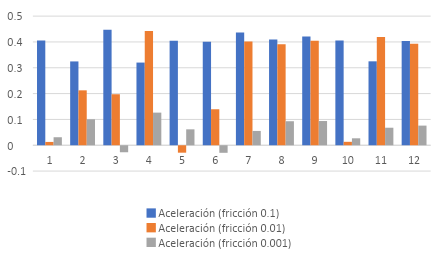
\includegraphics[scale=0.8]{aceleracion-friccion.png}
    \caption{Relación fricción - aceleración}
    \label{fig:friccion-acele}
\end{figure}

Por último, la Figura \ref{fig:vel-planoXZ} muestra la diferencia entre la progresión de la velocidad a lo largo del tiempo con y sin el motor de físicas complementario. Se observa que con el motor de físicas complementario la velocidad tarda unos milisegundos en estabilizarse y que cada vez se va ajustando mejor al valor objetivo. Sin embargo, la curva que genera la simulación sin el motor complementario es absolutamente irreal, ya que se está asuminedo una aceleración infinita.

\begin{figure}[h!]
    \centering
    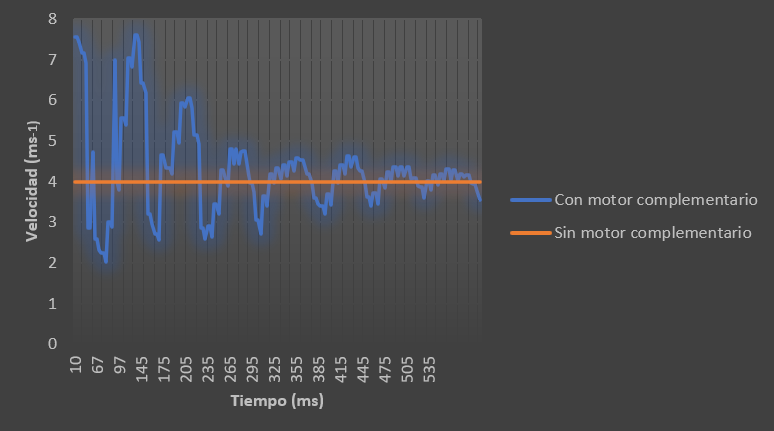
\includegraphics[scale=0.8]{PD_vel_XZ.PNG}
    \caption{Tiempo - Velocidad Controlador PD en velocidad del plano horizontal}
    \label{fig:vel-planoXZ}
\end{figure}

\newpage
\subsection{Simulación realista de drones}
El motor de físicas complementario dota a \textit{WebSim} de unas físicas más realistas puesto que permite a \textit{CANNON} materializar la gravedad. Gracias a ello, se pueden simular mundos en los que, a pesar de existir una gravedad de -9.8, la fuerza autónoma que hace aplicar el motor complementario permite volar al drone. \newline

Las físicas realistas implementadas permiten diferenciar entre el despegue de un drone ligero y el de uno mucho más pesado. Por ejemplo, para un fuerza máxima de 1 N, un drone de 1 Kg podrá despegar mientras que otro de 100 Kg no será capaz puesto que la fuerza máxima aplicada no es suficiente para superar la fuerza de la gravedad\footnote{\url{https://www.youtube.com/watch?v=S1E1zKjFkLo}}.

\begin{figure}[h!]
  \centering
  \begin{subfigure}[b]{\textwidth}
    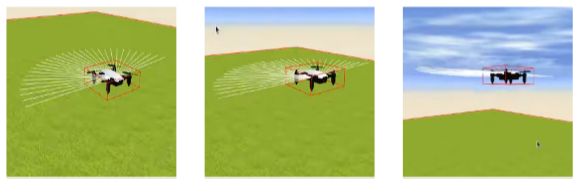
\includegraphics[scale=0.8]{masadrone_1.png}
    \caption{Despegue del drone Tello de 1 Kg}
  \end{subfigure}
  \hfill
  \begin{subfigure}[b]{\textwidth}
    \includegraphics[scale=0.8]{dronemasa_2.png}
    \caption{Despegue del drone Tello de 100 Kg}
  \end{subfigure}
\caption{Despegue con drones de diferentes masas}
\label{fig:masadrone}
\end{figure}


Por otro lado, el control PD en posición incrementa el realismo de las físicas también a nivel visual puesto que hace recrear un movimiento más fluido y no produce una brusca frenada como ocurría con la imposición de la posición con \textit{updatePosition}. La fluidez del movimiento se consigue gracias a la fase de estabilización característica del controlador PD hasta que consigue aproximar su salida al valor de referencia\footnote{\url{https://www.youtube.com/watch?v=jSGI6KJbzTQ}}. En la Figura \ref{fig:pos-ejeY} se aprecia cómo el controlador tarda unos ms en estabilizar la posición y al principio la posición tiende a caer como consecuencia de la atracción de la gravedad. La Figura \ref{fig:vel-ejeY} muestra la progresión de la velocidad a lo largo del tiempo cuando el drone despega.

\begin{figure}[h!]
    \centering
    \includegraphics[scale=0.8]{PD_pos_Y.PNG}
    \caption{Tiempo - Posición Controlador PD en posición para la altura}
    \label{fig:pos-ejeY}
\end{figure}

\begin{figure}[h!]
    \centering
    \includegraphics[scale=0.8]{PD_vel_Y.PNG}
    \caption{Tiempo - Velocidad Controlador PD en velocidad del eje vertical}
    \label{fig:vel-ejeY}
\end{figure}



% NUEVOS EJERCICIOS %
%%%%%%%%%%%%%%%%%%%%%%%%%%%%%%%%%%%%%%%%%%%%%%%%%%%%%%%%%%%%%%%%%%%%%%%%%%%%%%%%
\chapter{Nuevos ejercicios}
\label{chap:nuevos_ejercicios} 

   
\section{Roomba}
\section{Aparcamiento}
\section{Sigue-líneas sofisticado}
\section{ Laberinto 3D para mBot}
\section{Laberinto para drone}
\subsection{Con señalización}
\subsection{Sin señalización}
\section{Fútbol competitivo}
\subsection{Evaluador}



% CONCLUSIONES %
%%%%%%%%%%%%%%%%%%%%%%%%%%%%%%%%%%%%%%%%%%%%%%%%%%%%%%%%%%%%%%%%%%%%%%%%%%%%%%%%
\chapter{Conclusiones}
\label{chap:conclusiones} 
En este apartado se recogen las conclusiones a las que se ha llegado tras la realización de este Trabajo Fin de Grado y se van a valorar los resultados obtenidos. De igual forma, tras exponer las conclusiones y valoraciones, se presentarán algunas interesantes líneas futuras para mejorar y completar la implementación realizada.
   
\section{Conclusiones y valoración de resultados}
El objetivo principal de este trabajo era crear un motor de físicas mejorado para \textit{WebSim} que estuviera basado en tecnologías web y que permitiese dotar al simulador robótico de unas físicas más realistas. Se ha cumplido de manera satisfactoria implementando un nuevo motor de físicas complementario que coexiste con \textit{CANNON}. Materializa la fuerza autónoma de los robots, dejando como tarea de \textit{CANNON} la materialización de la gravedad, la fricción y la restitución de la escena para esos mismos robots.\newline

Anteriormente, las físicas de los robots se implementaban por medio de la función \textit{updatePosition}, que imponía una posición y velocidad al robot sin tener en cuenta la gravedad, la fricción ni la restitución. Era un modelo cinemático donde se asumía que los robots adquirían instantáneamente la velocidad ideal que el software del robot ordenaba. En consecuencia, los robots no se movían de manera realista puesto que se estaba asumiendo una aceleración infinita. Sin embargo, el nuevo motor complementario sí permite un movimiento realista puesto que al ser complementario a \textit{CANNON}, no elimina el efecto que este introduce con la fuerza de gravedad, la fricción y las colisiones, abriendo un amplio abanico de nuevas posibilidades de simulación en \textit{WebSim}. \newline 

El nuevo motor complementario consta de dos niveles. El primero incluye varios controladores PD que se encargan de traducir las velocidades deseadas que le llegan al motor complementario cada 20 ms a la fuerza autónoma a aplicar al robot para que este las alcance. El segundo nivel es un modelo de fuerzas que, a partir de la definición de la masa y el momento de inercia del robot, calcula la aceleración y par resultantes al aplicar la fuerza autónoma decidida por el primer nivel.

Los dos puntos que se pedían para cumplir este principal objetivo también se han logrado en la implementación:

\begin{itemize}
    \item Materialización de robots con distinta masa y que recreen un movimiento autónomo realista, con una aceleración máxima limitada y capacidad de control acotada.
    
    Este requisito se ha logrado satisfacer mediante la definición de una serie de parámetros que caracterizan el movimiento del robot en un escenario y las físicas del mismo. Se deben configurar para cada ejercicio. Algunos de estos atributos son propios de \textit{A-Frame} y otros son parámetros del modelo de fuerzas del nuevo motor complementario. En la tabla \ref{fig:parametros} se incluía el detalle de cada uno de estos parámetros. \newline
    
    Además de una mejora visual ofreciendo un movimiento más fluido y realista, permite recrear nuevas posibilidades de simulación, como por ejemplo:
    
    \begin{itemize}
        \item [$-$] La variación de la fricción del escenario permite recrear escenarios tan diversos como una pista de hielo o un campo de fútbol por donde rueda la pelota y avanzan los robots.
        \item [$-$] La materialización de la gravedad hace que sea necesario ejercer una fuerza autónoma capaz de superar la fuerza de la gravedad y hacer ascender al drone. Los objetos en los mundos de drones ahora sí pueden tener gravedad, antes estaba anulada.
        \item [$-$] La variación de la masa de los robots implica que sea necesario ajustar el resto de parámetros. Por ejemplo, un robot más pesado deberá ejercer una fuerza más grande que un robot más ligero para alcanzar la misma velocidad.
        \item [$-$] Los escenarios podrán incluir rampas, ya que los robots terrestres podrán subirlas si se parametrizan de forma correcta los valores de fricción y fuerza autónoma máxima.
        \item [$-$] Los robots tienen velocidad lineal y angular límite, al contrario de lo que ocurría con el modelo anterior. 
        \item [$-$] Se rompe con la premisa de aceleración infinita que se ha mantenido hasta el momento por el hecho de no imponer instantáneamente la velocidad deseada. Se tiene una fuerza máxima y, por lo tanto, una aceleración máxima.
        \item [$-$] Por el hecho de que el motor sea complementario, \textit{CANNON} materializa en paralelo la restitución de las colisiones, permitiendo recrear movimientos más realistas como el golpeo de una pelota.
    \end{itemize}
    
    \item Coexistencia con el motor por defecto \textit{CANNON} y que no requiera la modificación de su código fuente.
    
    El segundo punto se consiguió satisfacer gracias a la correcta combinación en el tiempo entre ambos motores que permite que cada uno de ellos materialice la parte de las físicas que le compete de manera independiente y que trabajen en la misma escala. Para ello, fue necesario conocer el ritmo de ejecución de ambos motores. En el caso del nuevo motor complementario es de 20 ms puesto que se incluyó un \textit{timeout} para establecer ese ritmo. En el caso de \textit{CANNON} fue necesario el registro de un nuevo componente auxiliar en \textit{A-Frame} que se debe incluir en todas las escenas y que permite monitorizar el ritmo de ejecución del bucle de renderizado de \textit{A-Frame}. En cada iteración del bucle de renderizado, \textit{CANNON} actualiza las posiciones y velocidades de los objetos de la escena materializando su parte de la dinámica.
\end{itemize}

El segundo objetivo era crear varios ejercicios en la plataforma educativa Kibotics que sacasen partido del nuevo motor de físicas y fueran más atractivos para los niños. Este objetivo también se ha completado de manera satisfactoria mediante la creación de cuatro escenarios diferentes que explotan las nuevas físicas de realistas de diferentes formas.

\begin{itemize}
    \item Creación de escenarios multinivel gracias a la materialización de la fricción, que permite la subida de rampas: sigue-líneas con rampa y laberinto 3D para mBot.
    \item Recreación del movimiento efectuado por una pelota rodando gracias a la materialización de la fricción: fútbol competitivo.
    \item Materialización del vuelo de un drone en escenarios con gravedad -9.8: laberinto para drone.
    \item Materialización de las colisiones que permite ajustar el coeficiente de restitución para hacer más realistas los choques entre objetos y el golpeo de un balón: fútbol competitivo.
\end{itemize}


\section{Líneas futuras}
La implementación de este nuevo motor de físicas complementario ha supuesto un gran avance en el funcionamiento de \textit{WebSim}. No obstante, aún existen múltiples líneas abiertas que ayudarán a mejorar aún más el entorno \textit{Kibotics}.

\begin{itemize}
    \item Creación de ejercicios competitivos para cuatro jugadores. Por ejemplo, se propone como punto de partida la extensión del ejercicio de fútbol competitivo uno contra uno a un ejercicio competitivo de dos contra dos.
    \item Exploración del nuevo motor de físicas \textit{ammo.js} y extender la implementación del motor complementario en conjunción con este otro motor. En el futuro, \textit{A-Frame} pasará a utilizar el motor \textit{ammo.js} como motor de físicas por defecto, dejando a un lado el de \textit{CANNON} ya que se preveé que quede obsoleto en los próximos años.
    \item Adición de efectos de sonido a los ejercicios. Un aspecto que otorgaría aún más realismo al simulador sería la adición de audio en los mismos. Sería de especial interés en ejercicios como el del fútbol competitivo, en el que se podría añadir el efecto del sonido del chute al balón y el del público celebrando un gol.
\end{itemize}


\cleardoublepage

% BIBLIOGRAFIA %
%%%%%%%%%%%%%%%%%%%%%%%%%%%%%%%%%%%%%%%%%%%%%%%%%%%%%%%%%%%%%%%%%%%%%%%%%%%%%%%%
\chapter{Bibliografía}
\label{chap:bibliografia} 

\end{document}